\documentclass[adraft,hidelinks]{eptcs}
\usepackage{_controlSequences}   % control sequences
\usepackage{comment}
\usepackage{underscore}
\usepackage{latexsym}
\usepackage{wrapfig}
\usepackage{marvosym}
\usepackage{color}
\usepackage{graphicx}
\usepackage{amsmath,amsfonts,amssymb}
\usepackage{stmaryrd}
\usepackage{multicol}
%\usepackage{enumitem}
\usepackage[shortlabels]{enumitem}
%  \setlist[enumerate, 1]{(1)}
\usepackage{framed,color}
\usepackage[utf8]{inputenc}
\definecolor{shadecolor}{rgb}{1,0.5,0.5}

\begin{document}

\def\titlerunning{Expressiveness}
\def\authorrunning{Anran Wang}
\title{\Large Expressiveness of Process Algebras with Signals, Broadcast, and Priorities}
\author{Anran Wang}
\maketitle

\tableofcontents

%%%%%%%%%%%%%%%%%%%%%%%%%%%%%%%%%%%%%%%%%%%%%%%%%%%%%%%%%%%%%%%%%%%%%%%%%%%%%%
%\input{01introduction.tex}
\section{Introduction}

Since its appearance in 1982, the \emph{Calculus of Communicating Systems (CCS)} \cite{RM80} has been studied, compared with other calculi, and equipped with more mechanisms.
The resulting new algebras can model certain distributed systems in a more precise and straightforward fashion, but also raise a question: do they only change the written form of the models, or are they truly more expressive than pure CCS?

Expressiveness in this context means the ability of a language to model, represent, portray entities, systems, protocols, etc.
If the expressiveness is described in a direct way, such as ``CCS can model addition", then it is called \emph{absolute expressiveness}.
If it is described comparatively, such as ``A is more expressive than B'', then it is called \emph{relative expressiveness}.
To compare the expressiveness of different calculi, one usually takes two approaches: for positive results, one \emph{encodes} one language into another.
Once such an encoding is established, one can infer that the target language is at least as expressive as the source.
Since each term in the source language can be encoded into a term in the target language, every model described in the source can therefore also be described in the target language.
To decide how ``good" the encoding is, one refers to \emph{encodability criteria}, which describe how structured the encoding is, how many behaviours it preserves, etc.
The criteria play an essential rule in expressiveness studies.
An encoding can be treated as ``good'' due to some set of criteria, but fails to conform to another set that is either more strict or totally different.
%A separation result can be nullified by a set of looser criteria, even if it can separate two algebras with more strict criteria.
%In other words, the looser the criteria are, the stronger the separation results are.

For negative results, one searches for \emph{separation results}.
If one can find a system, algorithm, etc. that can be modelled by one algebra but not by another, one can conclude that this separates the two algebras, and the first algebra cannot be expressed by the other.
%If there is an encoding from algebra A to algebra B, and separation result from B to A, then B is strictly more expressive than A.
%If there are separation results from A to B and vice versa, then A and B are incomparable when it comes to expressive power.

In this \this, we first present at the beginning of Section \ref{definition} some relevant definitions.
The syntax and semantics of the process algebras to be explored are explained in Sections \ref{sec:ccs}, \ref{sec:ccss}, \ref{sec:abc}, and \ref{sec:ccssg}, introducing CCS, CCS with Signals (CCSS), the Algebra of Broadcast Communication (ABC), CCS with Priorities (\CSG), respectively.

Expressiveness criteria consulted in this thesis are listed in \Sec{criteria}.
Encodings are given in \Sec{ccs-ccss} from CCS to CCSS/ABC/\CSG and vise versa.
Separation results are exhibited in \Sec{ccss-ccs} as well as \Sec{abc-ccs} concerning CCSS and ABC, respectively.
We proceeded to an encoding from ABC to \CSG in \Sec{abc-ccssg}.
In the end, we separated \CSG from other calculi in \Sec{ccssg-ccs}.

Finally, a map of relative expressive power is shown in \Sec{conclusion}.

%%%%%%%%%%%%%%%%%%%%%%%%%%%%%%%%%%%%%%%%%%%%%%%%%%%%%%%%%%%%%%%%%%%%%%%%%%%%%%
%\input{02preliminaries.tex}
\section{Preliminaries: CCS and its Extensions with Signals, Broadcasts, and Priorities}
\label{definition}

In general, the symbol $\Name$ represents the set of all possible names.
%$\overline{\Name} := \{\overline{c}\mid c\in\Name\}$ while
$\K$ is the set of all possible agent identifiers, and $\St$ is the set of all possible process terms.

When $\Name$, $\K$, and $\St$ are equipped with indices, then the symbols indicate the subset of names, agent identifiers, and terms in the specific process algebra.
For example, $\Name_{CCS}\subseteq \Name$ is the subset of names that parameterise CCS.

\begin{definition}{lts}\textbf{(LTS)}
  A \emph{labelled transition system} (LTS) is a tuple $(\St, \Lab, \ar{})$ with $\St$ set of states, $\Lab$ set of labels.
  $\ar{}$ is a transition relation that is a subset of $\St\times\Lab\times\St$.
  The transition relation is usually written as $source\ar{label}\target$.

  An LTS is \emph{rooted} if there is a unique state $s_0$ called \emph{root}.
\end{definition}

\begin{definition}{reduction}\textbf{(Reduction)}
  The \emph{reduction relation} is a subset of a given transition relation, where the set of labels includes only \emph{reduction labels}.

  A transition is called a \emph{reduction} if it is labelled with an $l\in\Name_r$ and is written $source \ar{} target$.

  Formally, $P\ar{}Q$ if and only if $\exists \alpha\in\Name_r:\ P\ar{\alpha} Q$.
\end{definition}
Usually, the set of reduction labels $\Name_r$ only includes the silent action $\tau$, such as in CCS.
The set of reduction labels should only include labels of actions that can occur autonomously.
For instance, the action ``start'' of an automobile waiting at a crossroad should not be labelled with a reduction label, for it depends on the traffic light doing ``signal green''; the action ``signal green'', however, should be labelled with a label from $\Name_r$, because it happens according to its own logic, not dependenting on its surroundings; it is indifferent however many cars are waiting.


\begin{definition}{path}\textbf{(Path)}
	A \emph{path} in a labelled transition system $L$ is a sequence of transitions, where the target state of one transition is the source state of the next transition.
  A path $\pi$ is written in the form:
  \[ \pi:\ s_0\ar{\alpha_1}s_1\ar{\alpha_2}s_2\cdots\ar{\alpha_n}s_n\]
  for some $n\in\IN$, or
  \[ \pi:\ s_0\ar{\alpha_1}s_1\ar{\alpha_2}s_2\cdots\]
  if the path is infinite.
  The \emph{source} of a path is the first state in the path, noted as $source(\pi)$.
  We note ``the path \emph{of} $P$" if the source of the mentioned path is $P$.
  The states in the path satisfy $s_n\ar{\alpha_{n+1}}s_{n+1}$, for all relevant $n$.
  When $n=0$ the path contains only one state.

  A path is \emph{maximal}, if it is either infinite or ends in a state with no outgoing transitions in $L$.

  A path is a \emph{computation} if all transitions are reductions.
  A computation is maximal, if it as a path is maximal.
\end{definition}

\begin{definition}{barb}\textbf{(Barb)}
  A state $P\in\St$ \emph{exhibits barb} or \emph{barbs} $x\in\Name\dcup\overline{\Name}$, written $P\barb{x}$, if and only if $P\ar{x}$, where $P\ar{x}$ if and only if $\exists P'\in\St:\ P\ar{x}P'$.

  A path $\pi$ exhibits barb $x$, written $\pi\barb{x}$, if and only if there exists at least one state $s_i$ within $\pi$ such that $s_i\barb{x}$.
  The collection of barbs forms the set of observables for $\pi$, written $\Ob{\pi} = \{x \mid \pi\barb{x}\}$.

  A state $P$ \emph{weakly barbs} $x$, written $P\wbarb x$ if and only if $\exists P':\ (P \vred{}{P'}) \wedge (P' \downarrow x)$, where $\vred{}$ is the reflexive, transitive closure over the reduction relation $source\ar{}target$.

  $P\nbarb x$ if and only if $P$ does not barb $x$, $P\nwbarb x$ if and only if $P$ does not weakly barb $x$.

  %is the $P\vred{}P'$ if and only if there exists a computation from $P$ to $P'$.
\end{definition}

%This is inspired by the definition of ``success'' in \cite{DG10}, but since there is no success label in CCS-like languages, we use barb instead.

\begin{definition}{pg}\textbf{(Process Graph)}
  A \emph{process} is an element of the set $\St$ of process terms.
  Given a process algebra PA, all elements in $\St_{PA}$ are called PA processes.

  A \emph{process graph} of a process $P$ is a rooted labelled transition system $(\St, \Lab, \ar{}, P)$ where $P$ is the root, $\St$ is the set of process terms, $\Lab$ the set of labels a.k.a. process names, $\ar{}$ the transition relation.
  $P\ar{\alpha}P'$ means process $P$ can do an action $\alpha$ and reach state $P'$, which is also a process.
\end{definition}

\subsection{CCS: Calculus of Communicating Systems}
\label{sec:ccs}
The Calculus of Communicating Systems (CCS) \cite{RM80} is a process algebra parameterised with $\K_{CCS}$ and $\Name_{CCS}$.
The set of handshake actions is $\HS_{CCS} := \Name_{CCS}\dcup\overline{\Name_{CCS}}$ where $\overline{\Name_{CCS}} := \{\overline{c}\mid c\in\Name_{CCS}\}$, $\dcup$ is the disjoint union\footnote{The disjoint union $\dcup$ implies that the sets it joins are disjoint. },
$\overline{\cdot}$ denotes the complement of a name, it satisfies $\overline{\overline{c}} = c$ for $c\in\Name_{CCS}$ and $\overline{\tau} = \tau$, where $\tau$ is a special name not in $\Name_{CCS}$ nor $\Name$ that represents a silent action.
In CCS, $\tau$ is the only reduction label.

The set of actions $\Act_{CCS} := \HS_{CCS} \dcup \{\tau\}$.

In the remaining subsection, let $c$ range over $\HS_{CCS}$, $\alpha$ over $\Act_{CCS}$, $A$ over $\K_{CCS}$.
The class $\Sccs$ of CCS expressions is the smallest set including:
\begin{table*}[h]
\centering
\caption{CCS Expressions}
\label{CCSExp}
$\boxed{
  \begin{array}{ll}
    \bullet\ \  \text{\emph{prefixes\ \ }} \alpha.P &
    \hspace{5mm}\bullet\ \  \text{\emph{(infinite) choices\ \ }}  \sum_{i\in I} P_i \\
    \bullet\ \  \text{\emph{restrictions\ \ }} P\backslash L &
    \hspace{5mm}\bullet\ \  \text{\emph{parallel compositions\ \ }}  P|Q \\
    \bullet\ \  \text{\emph{relabellings\ \ }}  P[f] &
    \hspace{5mm}\bullet\ \  \text{\emph{agent identifiers\ \ }} A
  \end{array}}$
\end{table*}

\noindent where $P, Q\in\Sccs$, $A\in\K_{CCS}$, $I$ is an index set, $L\subseteq \Name_{CCS}$ a subset of names, $f: \HS_{CCS}\to\HS_{CCS}$ a renaming function satisfying $f(\overline{a}) = \overline{f(a)}$ and extends to $\Act_{CCS}$ by defining $f(\tau) = \tau$.
$\nil$ (nil) represents inaction, defined as $\nil := \sum_{i\in \emptyset} P_i$.
%$S: \V_{CCS}\to \Sccs$ is a recursion specification, with $\V_S\subseteq\V_{CCS}$ the domain of $S$. Sometimes a recursion specification is written as $\{Y = S(Y) | Y\in\V_S\}$.
In case $i\in\{1,2\}$, we write $P_1+P_2$ instead of $\sum_{i\in\{1,2\}}P_i$ for readability.

In CCS as well as its extentions, each agent identifier comes with a defining equation $A \defis P$ where $P$ is a CCS term and does not contain occurrances of \emph{unguarded} agent identifiers.
An agent identifier $A$ is guarded, if there is $\alpha\in\Act_{CCS}$ as prefix of $A: \alpha.A$.
Otherwise it is unguarded.
The same is required for agent identifiers in CCSS, ABC, and \CSG.

The symbol $\defis$ is in principle the same as $:=$, we use it to emphasise the (possible) appearance of recursions.
Recursions are defined using agent identifiers, for example $P \defis \alpha.P$ is a process that does action $\alpha$ repeatedly.


Let $\St=\St_{CCS}$, $\Lab=\Act_{CCS}$ in \df{lts}, CCS yields a labelled transition system.
Based on LTS, the semantics of an algebra can be given by means of \emph{structural operational semantics (SOS)}.
A rule in an SOS table takes the following form:
\[ \frac{\text{set of condition(s)}}{\text{set of result(s)}}\]

This rule means ``if the conjunction of the conditions is true, then the results can happen''.
When the set of conditions in an SOS rule is empty, this rule is called an \emph{axiom}, and the results can always happen.

All CCS transitions follow the rules in Table \ref{tab:CCSsos}.

\begin{table*}[t]
\normalsize
\centering
\caption{Structural Operational Semantics of CCS}
\label{tab:CCSsos}
\framebox{
$\begin{array}{@{}ccc@{}}
\displaystyle\frac{}{\alpha.\E \ar{\alpha} \E}  \mylabel{act}&
%\\[3ex]
\displaystyle\frac{\E_j \ar{\alpha} \E',\ j\in I}{\sum_{i\in I} \E_i \ar{\alpha} \E'}  \mylabel{sum}
\\[3ex]
\displaystyle\frac{\E\ar{\alpha} \E'}{\E|\F \ar{\alpha} \E'|\F} \mylabel{par-l}&
\displaystyle\frac{\F\ar{\alpha} \F'}{\E|\F \ar{\alpha} \E|\F'} \mylabel{par-r}&
\displaystyle\frac{\E\ar{{c}} \E', ~\F \ar{\bar{{c}}} \F'}{\E|\F \ar{{\tau}} \E'| \F'} \mylabel{comm}
\\[3ex]
\displaystyle\frac{\E \ar{\alpha} \E'}{\E[f] \ar{f(\alpha)} \E'[f]} \mylabel{rel}&
\displaystyle\frac{\E \ar{\alpha} \E', \alpha,\bar{\alpha}\notin L}{\E\backslash L \ar{\alpha} \E'\backslash L} \mylabel{res}&
\displaystyle\frac{\E \ar{\alpha} \E'}{A\ar{\alpha}\E'} (A\defis\E) \mylabel{rec}
\end{array}$}
\end{table*}


\subsection{CCS with Signals}
\label{sec:ccss}
CCS with Signals (CCSS) \cite{DvGH17} is acquired by extending CCS with a set of \emph{signals} as well as a \emph{siganlling} operator.
The set of names in CCSS is defined as $\Name_{CCSS} := \Name_{CCS} \dcup \Sig$ where $\Sig$ is the set of signals.
Note that the only names in $\Name_{CCS}$ have complement.

The set of handshake actions is $\HS_{CCSS} := \HS_{CCS}$.
The set of actions in CCSS is defined by $\Act_{CCSS} := \Sig \dcup \HS_{CCSS} \dcup \{\tau\}$.
The set of agent identifiers $\K_{CCSS}:=\K_{CCS}$.

The binary operator signalling binds a CCSS process $P$ and a signal $s$ in such form: $P\signals s$.

The class $\St_{CCSS}$ of CCSS expressions is the smallest set including:
\begin{table*}[h]
\centering
\caption{CCSS Expressions}
\label{CCSSExp}
$\boxed{
  \begin{array}{lll}
    \bullet\ \  \text{\emph{prefixes\ \ }} \alpha.P &
    \hspace{5mm}\bullet\ \  \text{\emph{(infinite) choices\ \ }}  \sum_{i\in I} P_i &
    \hspace{5mm}\bullet\ \  \text{\emph{signalling\ \ }}  P\signals s \\
    \bullet\ \  \text{\emph{restrictions\ \ }} P\backslash L &
    \hspace{5mm}\bullet\ \  \text{\emph{parallel compositions\ \ }}  P|Q \\
    \bullet\ \  \text{\emph{relabellings\ \ }}  P[f] &
    \hspace{5mm}\bullet\ \  \text{\emph{agent identifiers\ \ }} A
  \end{array}}$
\end{table*}

where $\alpha\in\Act_{CCSS}$, $I$ an index, $P,Q\in\St_{CCSS}$, $A\in\K_{CCSS}$, $s\in\Sig$, $L\subseteq \Name_{CCSS}$, $f:(\Sig\to\Sig)\cup(\HS_{CCSS}\to\HS_{CCSS})$ satisfying $f(\overline{a}) = \overline{f(a)}$, it extends to $\Act_{CCSS}$ by defining $f(\tau) = \tau$.

The semantics of CCSS is extended from Table \ref{tab:CCSsos} with Table \ref{tab:CCSSsos}.
The curved arrow symbol $\sigar{}$ indicates the ability of a CCSS process to emit signals.
The collection of reduction labels in CCSS is $\{\tau\}$.

\begin{table}[t]
\caption{Structural Operational Semantics of Signals in CCSS}
\normalsize
\begin{center}
  \framebox{$\begin{array}{cccc}
  (P \signals s)\sigar{s}&
  \displaystyle\frac{P\ar{\alpha}P'}{P\signals r \ar{\alpha}P'}&
  \displaystyle\frac{{P_i}\sigar{s},\ i\in I}{\sum_{i\in I}P_i \sigar{s}}&
  \\[4ex]
  \displaystyle\frac{P\sigar{s}}{(P|Q) \sigar{s}} &
  \displaystyle\frac{P\sigar{s},~ Q \ar{s} Q'}{P|Q \ar{\tau} P| Q'} &
  \displaystyle\frac{P\ar{s}P',~ Q \sigar{s}}{P|Q \ar{\tau} P'| Q}&
  \displaystyle\frac{Q\sigar{s}}{(P|Q) \sigar{s}}\\[4ex]
  \displaystyle\frac{P\sigar{s}}{(P\signals r)\sigar{s}}&
  \displaystyle\frac{P \sigar{s}}{(P\backslash \RL) \sigar{s}}~~(s\not\in\RL) &
  \displaystyle\frac{P \sigar{s}}{P[f] \sigar{f(s)}} &
  \displaystyle\frac{P \sigar{s}}{A\sigar{s}}~~(A \stackrel{{\it def}}{=} P)
  \end{array}$}
\end{center}
\label{tab:CCSSsos}
\end{table}

\subsection{Algebra of Broadcast Communication}
\label{sec:abc}
The Algebra of Broadcast Communication (ABC) \cite{vGH15} is an extension of CCS, combined with features from the Calculus of Broadcasting Systems (CBS) \cite{KP91}.

The set of names in ABC is extended with broadcast names $\B$, they are sometimes called \emph{channels}.
The sets of \emph{broadcast} and \emph{receive} actions are given by $\B\sharp = \{b\sharp \mid b\in\B\}$ where $\sharp\in\{!, ?\}$.
The exclamation mark $!$ is the notation for broadcasting and the question mark $?$ for receiving.
As a result, $\Name_{ABC} := \Name_{CCS}\dcup\B$, $\Act_{ABC} := \HS_{ABC}\dcup\B!\dcup\B?\dcup\{\tau\}$ where $\HS_{ABC} := \HS_{CCS}$.
A relabelling function is $f: (\B\to\B) \cup (\Name_{CCS}\to\Name_{CCS})$, it extends to $\Act_{ABC}$ by $f(\overline{c}) = \overline{f(c)}$, $f(b\sharp) = f(b)\sharp$, $f(\tau) = \tau$.
The set of agent identifiers in ABC $\K_{ABC}:=\K_{CCS}$.

Note that only names in $\B$ have complement.

The class of ABC terms is defined by Table \ref{CCSExp}, where $\alpha\in\Act_{ABC}$, $L\subseteq \HS_{ABC}$\footnote{This implies that neither silent nor broadcast actions can be restricted. }, $f$ a relabelling function, $P, Q\in\St_{ABC}$, and $A\in\K_{ABC}$.

The semantics of ABC is extended from \tab{CCSsos} with rules in Table \ref{tab:ABCsos}, where $\sharp_1$, $\sharp_2$, $\sharp \in \{!, ?\}$.

The reduction relation in ABC is defined as $\{\tau\}\cup\B!$, considering broadcast actions happen autonomously, and should not be blocked in any way.

\begin{table*}[t]
\normalsize
\centering
\caption{Structural Operational Semantics of ABC}
\label{tab:ABCsos}
\framebox{
$\begin{array}{@{}ccc@{}}
\!\displaystyle\frac{\E\ar{b\sharp_1} \E' ,~ \F \nar{b?}}{\E|\F \ar{b\sharp_1} \E'| \F}  \mylabel{Bro-l}&
\displaystyle\frac{\E\ar{b\sharp_1} \E' ,~ \F \ar{b\sharp_2} \F'}{\E|\F \ar{b\sharp} \E'| \F'} \mylabel{Bro-c} \\[3ex]
\displaystyle\frac{\E\nar{b?} ,~ \F \ar{b\sharp_2} \F'}{\E|\F \ar{b\sharp_2} \E| \F'}  \mylabel{Bro-r}%\\[-5pt]
& \scriptstyle \sharp_1\circ\sharp_2 = \sharp \neq \_ ~~\mbox{with}~~
    \begin{array}{c@{\ }|@{\ }c@{\ \ }c}
    \scriptstyle \circ & \scriptstyle ! & \scriptstyle ? \\
    \hline
    \scriptstyle ! & \scriptstyle \_ & \scriptstyle ! \\
    \scriptstyle ?& \scriptstyle ! & \scriptstyle ? \\
    \end{array}
\\[1ex]
\end{array}$}
\end{table*}

\subsection{CCS with Priorities}
\label{sec:ccssg}
Cleaveland, Lüttgen, and Natarajan categorised process-algebraic priorities by combining its two characteristics: \emph{static} or \emph{dynamic priorities}, and \emph{local} or \emph{global preemption} \cite{CLN01}.
In this \this, we are going to look into CCS with static priority and global preemption, noted as $CCS^{sg}$ \cite{CLN01}.

The names in \CSG always include a priority level.
%The complement operator is defined over $\Name_{CCS^{sg}}$.
A prioritised name is of the form $a\cln k$ or $\overline{a\cln k}$ where $k\in\IN$ is a priority level, with $0$ being the highest.
The set of \CSG names is $\Name_{CCS^{sg}} := \{a\cln k \mid a\in\Name_{CCS},\ k\in\IN\}$, $\overline{\Name_{CCS^{sg}}} := \{\overline{a\cln k} \mid a\cln k\in\Name_{CCS^{sg}}\}$.
Additionally, the complementat of a name satisfies $\overline{\alpha\cln k} = \overline{\alpha}\cln k$.
The set of agent identifiers $\K_{CCS^{sg}} := \K_{CCS}$.

Any relabelling function $f: \Name_{CCS}\to\Name_{CCS}$ extends to \CSG names by defining $f(\alpha\cln k):=f(\alpha)\cln k$ for $\alpha\in\Name_{CCS}$ and $k\in\IN$ a priority level.
Note that relabelling functions do not change priority levels.

The restricted set $L_p\subseteq \Name_{CCS^{sg}}$ and $\overline{L_p}:=\{\overline{\alpha\cln k} \mid \alpha\cln k\in L_p \}$.

The sets of handshake actions and actions are defined in \CSG similarly as in CCS, $\HS_{CCS^{sg}} := \Name_{CCS^{sg}} \dcup \overline{\Name_{CCS^{sg}}}$, $\Act_{CCS^{sg}} := \HS_{CCS^{sg}} \dcup \{\tau\cln k\mid k\in \IN\}$.
The set of reduction relations is the set containing silent actions with all priorities: $\{\tau\cln k\mid k\in \IN\}$.

Note that co-names have the same priorities , i.e. the co-name of $a\cln 0$ and the co-name of $a\cln 1$ are different.
In fact, actions with different priorities do not communicate.

To illustrate the operational semantics of \CSG, we need to first build \emph{potential initial action sets} $I$, as shown in Table \ref{tab:pias} ($k\in\IN$).
Intuitively, the potential initial action sets include actions that a process can perform according to SOS rules of CCS.
At this stage we do not consider the possibility that some actions may be preempted (\df{pree}) by others, thus the actions are \emph{potential}.
The potential initial action set of a process is built merely upon the structure of the process, thus \emph{initial}.

In \tab{pias}, the set $\overline{I(P)}$ is defined as $\overline{I(P)} := \{\overline{a\cln k} \mid a\cln k \in I(P)\}$,
$P\backslash L_P$ is restriction in \CSG, and $I(P)\backslash(L_p\cup\overline{L_p})$ is the usual set substraction.
%$I^{<l} := \underset{k<l}{\bigcup}I^k$, and thus $I^{<0} = \emptyset$.

\begin{table*}[t]
\normalsize
\centering
\caption{Potential Initial Action Sets for \CSG}
\label{tab:pias}
\framebox{
$\begin{array}{ll}
I(\alpha\cln k.P) := \{\alpha\cln k \} &
I(P[f]) := \{f(\alpha\cln k) \mid \alpha\cln k \in I(P)\}
\\[1ex]
I(P\backslash L_p) := I(P)\backslash(L_p\cup\overline{L_p}) &
I(\sum_{i\in I} P_i) := \underset{i\in I}{\bigcup} I(P_i) \text{ ($I$ an index set)}
\\[1ex]
I(A) := I(P)\ (A\defis P) &
I(P | Q) := I(P)\cup I(Q)\cup\{\tau\cln k \mid I(P)\cap \overline{I(Q)} \neq \emptyset\}
\end{array}$}
\end{table*}

When an action has the highest priority, its operational semantics coincide with Table \ref{tab:CCSsos}, but we still include it in the left side of Table \ref{tab:CCSsgsos} for readability.
When an action has priority $0 < l$, it can only happen when not preempted (\df{pree}) by a higher prioritised $\tau\cln k$, as represented in the right side of Table \ref{tab:CCSsgsos} ($0<l, k<l$, $I$ is an index set, $\alpha\cln 0$, $\alpha\cln l\in\Act_{CCS^{sg}}$, $c$, $\overline{c}\in \HS_{CCS^{sg}}$).

\begin{table*}[t]
\normalsize
\centering
\caption{Structural Operational Semantics of \CSG}
\label{tab:CCSsgsos}
\framebox{
$\begin{array}{@{}cc@{}}
\displaystyle\frac{}{\alpha\cln 0.\E \ar{\alpha:0} \E} &
\displaystyle\frac{}{\alpha\cln l.\E \ar{\alpha:l} \E}
\\[3ex]
\displaystyle\frac{\E_j \ar{\alpha:0} \E',\ j\in I}{\sum_{i\in I}\E_i \ar{\alpha:0} \E'} &
\displaystyle\frac{\E_j \ar{\alpha:l} \E',\ j\in I, \forall i\neq j\ \forall k<l: \tau \cln k \notin I(P_i)}{\sum_{i\in I}\E_i \ar{\alpha:l} \E'}
\\[3ex]
\displaystyle\frac{\E\ar{\alpha:0} \E'}{\E|\F \ar{\alpha:0} \E'|\F} &
\displaystyle\frac{\E\ar{\alpha:l} \E', \forall k<l:\tau \cln  k \notin I(\E|\F)}{\E|\F \ar{\alpha:l} \E'|\F}
\\[3ex]
\displaystyle\frac{\F\ar{\alpha:0} \F'}{\E|\F \ar{\alpha:0} \E|\F'} &
\displaystyle\frac{\F\ar{\alpha:l} \F', \forall k<l: \tau \cln  k \notin I(\E|\F)}{\E|\F \ar{\alpha:l} \E'|\F}
\\[3ex]
\displaystyle\frac{\E\ar{{c:0}} \E', ~\F \ar{\overline{{c:0}}} \F'}{\E|\F \ar{{\tau:0}} \E'| \F'} &
\displaystyle\frac{\E\ar{{c:l}} \E', ~\F \ar{\overline{{c:l}}} \F', \forall k<l: \tau \cln  k \notin I(\E|\F)}{\E|\F \ar{{\tau:l}} \E'| \F'}
\\[3ex]
\displaystyle\frac{\E \ar{\alpha:0} \E'}{\E[f] \ar{f(\alpha:0)} \E'[f]} &
\displaystyle\frac{\E \ar{\alpha:l} \E'}{\E[f] \ar{f(\alpha:l)} \E'[f]}
\\[3ex]
\displaystyle\frac{\E \ar{\alpha:0} \E', \alpha \cln  0, \overline{\alpha \cln  0} \notin L_p}{\E\backslash L_p \ar{\alpha:0} \E'\backslash L_p} &
\displaystyle\frac{\E \ar{\alpha:l} \E', \alpha \cln  l, \overline{\alpha \cln  l} \notin L_p}{\E\backslash L_p \ar{\alpha:l} \E'\backslash L_p}
\\[3ex]
\displaystyle\frac{\E \ar{\alpha:0} \E'}{A\ar{\alpha:0}\E'} (A\defis\E) &
\displaystyle\frac{\E \ar{\alpha:l} \E'}{A\ar{\alpha:l}\E'} (A\defis\E)
\end{array}$}
\end{table*}

\begin{definition}{pree}
  A process $P$ preempts the execution of $\alpha\cln l$, if and only if $P\ar{\tau:k}\, \wedge\  k<l$.
\end{definition}

So far we have established different sets of names, Figure \ref{fig:names} helps clear the relationship between the sets.

\begin{figure}[ht]
  \centering
  \caption{Names in CCS as well as its Extensions}
  \includegraphics[width = 0.5\textwidth]{images/names.pdf}
  \label{fig:names}
\end{figure}

The structural congruence relation ${\equiv}\in\St_{AG}\times\St_{AG}$, where $AG\in\{$CCS$,\ $CCSS$,\ $ABC$,\ $\CSG$\}$, is the smallest relation defined with the axioms in Table \ref{tab:syneq}, for all $x\in\St_{AG}$. %satisfying alpha conversion.
Also, we write $x.\nil$ as $x$ for short.

\begin{table*}[t]
\centering
\caption{Syntactic Equality Relation in CCS, CCSS, ABC, \CSG}
\label{tab:syneq}
\framebox{
$\begin{array}{lll}
  %x.\nil = x &
  x + \nil \equiv x &
  %\nil.x = \nil &
  x|\nil \equiv x \\
  x + x \equiv x &
  x + y \equiv y + x &
  x | y \equiv y | x \\
\end{array}$
}
\end{table*}
%TODO: change = to \equiv at some places.


%%%%%%%%%%%%%%%%%%%%%%%%%%%%%%%%%%%%%%%%%%%%%%%%%%%%%%%%%%%%%%%%%%%%%%%%%%%%%%
%\input{03expressiveness.tex}
\section {Expressiveness of CCS, CCSS, ABC, and CCS$^{sg}$}
\label{sec:expre}

\subsection{Expressiveness Criteria}
\label{sec:criteria}
Now we will explore the relative expressiveness of the aforementioned process algebras by constructing encodings or finding separation results.
We establish some expressiveness criteria in this subsection, but readers are encouraged to read \df{encd} then skip the following pages to \Sec{ccs-ccss} and refer back when the encodability criteria are consulted.

In his survey \cite{JP08}, Parrow gave an overview on approaches to explore expressiveness, as well as many feasible criteria, some of which are applicable for the purpose of this \this.
Gorla summarised some widely accepted criteria in \cite{DG10}, part of them are also used for this \this.
Also, the criteria used by Ene and Muntean \cite{EM99}, Versari, Busi and Gorrieri \cite{VBG09}, Phillips \cite{IP08} are applied here.

\begin{definition}{encd}\textbf{(Encoding)}
  An \emph{encoding} is a pair $(\bkt{\ }, \varphi_{\bkt{}})$ where $\bkt{\ }$ is a mapping $\St_1\to\St_2$ from the set of process expressions (process terms) $\St_1$ in the source language to the set of process terms $\St_2$ of the target language.
  $\varphi_{\bkt{}}$ is a \emph{renaming policy} $\Name\to\Name^k$ such that when $u\neq v$, $\ren{u}=(u_1, u_2, \dots, u_k)$, $\ren{v}=(v_1, v_2, \dots, v_k)$: $\forall i,j\in\{1,2,\dots, k\}, \nexists u_i=v_j$.
\end{definition}

In most cases, a name in the source language is simply translated to itself; in some cases, a name is translated to another name.
Either way, we omit the situation where a name is translated to a tuple of names and define the renaming policy as $\varphi_{\bkt{}}: \Name\to\Name$.

Since there is now only one element in both $\ren{u}$ and $\ren{v}$, $\ren{u}$ and $\ren{v}$ share no common element (when $\ren{u} \neq \ren{v}$) implies that $\ren{}$ is injective.

\begin{criterion}{comp}
  An encoding is \emph{compositional}, if for each $k$-ary operator $g$ in the source language, there exists a $k$-ary context $C_k(p_1, \dots, p_k)$ in the target language such that
  $\bkt{g(s_1, \dots, s_k)} = C_k(\bkt{s_1}, \dots, \bkt{s_k})$, where $p_1,\dots,p_k$ stand for ``holes" in the context to be filled with a concrete process.
\end{criterion}

\begin{criterion}{homo}
  An encoding is \emph{homomorphic} with respect to an operator $g$, if there is an identical operator in the target language, so that $\bkt{g(s_1, \dots, s_k)} = g(\bkt{s_1}, \dots, \bkt{s_k})$.

  Homomorphy is a special case of compositionality.
\end{criterion}


\begin{criterion}{corr} \cite{EM99, DG10}
  An encoding is \emph{operational correspondent} up to a relation $\eqv_2$ if it satisfies:
\begin{itemize}
  \item[1.] \mylabel{complete} if $S\vred{}_1S'$ then $\bkt{S}\vred{}_2{\eqv_2}\bkt{S'}$; and
  \item[2.] \mylabel{sound} if $\bkt{S}\vred{}_2 {\eqv_2}\bkt{T}$ then $S\vred{}_1S' \wedge \bkt{S'}{\eqv_2}\bkt{T}$ for some $S'$\footnote{This criterion is incomparable with Gorla's criterion named ``sound", and weaker than the criteria used by Ene and Muntean for ``uniform encoding".}.
\end{itemize}

\end{criterion}

${\eqv_i}\subseteq\St_i\times\St_i$ is an equivalence relation, $\vred{}_i$ (Definition \ref{df:barb}) is defined as the reflexive, transitive closure over the reduction relation $\ar{}_i$.
$P\vred{}_i\eqv_i Q$ if and only if $\exists P'\in\St_i: P'\eqv_i Q$.

The index indicates relations in the source or target language.
We omit the use of indices if there is no confusion.

\begin{criterion}{divref} \cite{DG10}
	An encoding with $\bkt{\ }$: $\St_1 \to \St_2$ \emph{reflects divergence} if and only if \[\forall S\in\St_1: \bkt{S} \divg_2\text{ implies } S \divg_1.\]

  $P\divg_i$, $i\in\{1,2\}$, if and only if there exists an infinite computation that has $P$ as its source, and we say $P$ is \emph{divergent}.
\end{criterion}

\begin{lemma}{div}
  If the encoding $\enc$ reflects divergence, and the process $P\in\St_1$ is not divergent, then $\bkt{P}$ is also not divergent.
\end{lemma}

\begin{proof}
  Directly from Criterion \ref{crt:divref}.
\end{proof}

\begin{criterion}{obsres} \cite{IP08, VBG09}
  Given a set of observables (Definition \ref{df:barb}) $Obs\subseteq\Name\dcup\overline{\Name}$, an encoding with $\bkt{\ }: \St_1\to\St_2$ is:
  \begin{enumerate}
    \item \label{sobsres} \emph{observation-respecting} if $\forall P \in \St_1$:
      \begin{itemize}
        \item[--] for every maximal computation (Definition \ref{df:path}) $\C$ of $P$ there exists a maximal computation $\C'$ of $\bkt{P}$ such that $\Ob{\C} = \Ob{\C'}$ (\df{barb}); and
        \item[--] for every maximal computation $\C'$ of $\bkt{P}$ there exists a maximal computation $\C$ of $P$ such that $\Ob{\C'} = \Ob{\C}$.
      \end{itemize}
    \item \label{wobsres} \emph{weakly observation-respecting} if $\forall P \in \St_1$:
      \begin{itemize}
        \item[--] for every maximal computation $\C$ of $P$ there exists a maximal computation $\C'$ of $\bkt{P}$ such that $\Ob{\C} = \Ob{\C'}$; and
        \item[--] for every maximal computation $\C'$ of $\bkt{P}$ there exists a maximal computation $\C$ of $P$ such that $\Ob{\C'} \subseteq \Ob{\C}$.
      \end{itemize}
  \end{enumerate}
\end{criterion}

Informally, when an encoding is observation-respecting, any encoded term exhibits exactly so many observables as its source term; when an encoding is weakly observation-respecting, the encoded term are not allowed to exhibit more observales as its source term.

\begin{criterion}{presem} \cite{JP08}
  An encoding \emph{preserves semantics} w.r.t. a behavioural equivalence $\asymp\,\ \subseteq\,  ((\St_1\cup\St_2)\times(\St_1\cup\St_2))$, if the encoded term satisfies:
  \[
    \forall P \in \St_1: \bkt{P} \asymp P.
  \]
\end{criterion}

This criterion is applicable, when the source and target algebras are similar, and there are equivalence relations defined over the union of the sets of source and target terms.

\emph{Strong bisimulation} can be considered as one such equivalence relation.

\begin{definition}{sbisim}\textbf{(Strong Bisimulation)}
  Let $P, Q\in\St$ be two processes, $\alpha$ is an action.
  $P$, $Q$ are \emph{strongly bisimilar} iff there is exists a binary relation $\RB$ over $\St$ such that
  \begin{enumerate}[label=(\roman*)]
    \item if $P\RB Q$ then $\forall P\ar{\alpha}P':$ $\exists Q'$ s.t. $Q\ar{\alpha}Q' \wedge P'\RB Q'$;
    \item if $P\RB Q$ then $\forall Q\ar{\alpha}Q':$ $\exists P'$ s.t. $P\ar{\alpha}P' \wedge P'\RB Q'$;
  \end{enumerate}
  The relation $\RB$ is called a \emph{strong bisimulation relation}.
\end{definition}

A superset of the set of strong bisimulation relations is the set of \emph{weak bisimulation} relations.

\begin{definition}{wbisim}\textbf{(Weak Bisimulation)}
  Let $P, Q\in\St$ be two processes, $\alpha$ is an action.
  $P$, $Q$ are \emph{weakly bisimilar} iff there is exists a binary relation $\RB$ over $\St$ such that
  \begin{enumerate}[label=(\roman*)]
    \item if $P\RB Q$ then $\forall P\ar{\alpha}P':$ $\exists Q'$ s.t. $Q\vred{\hat{\alpha}}Q' \wedge P'\RB Q'$;
    \item if $P\RB Q$ then $\forall Q\ar{\alpha}Q':$ $\exists P'$ s.t. $P\vred{\hat{\alpha}}P' \wedge P'\RB Q'$;
  \end{enumerate}
  where
  $\vred{\hat{\alpha}}:=
  \begin{cases}
    \vred{}\ar{\alpha}\vred{}, & \text{, if }\hat\alpha\neq\hat\tau\\
    \vred{} & \text{, else}
  \end{cases}$

  The relation $\RB$ is called a \emph{weak bisimulation relation}.
\end{definition}

Strong bisimulation relations are \emph{finer} than weak bisimulation relations.

\begin{definition}{finer}
  An equivalence relation ${\eqv_a}\subseteq \St\times\St$ is \emph{finer} than ${\eqv_b}\subseteq \St\times\St$, if and only if for all $P, Q\in\St$, $P\eqv_a Q$ implies $P\eqv_b Q$, and there exists $P'$, $Q'\in\St:$ $P'\eqv_b Q' \wedge P'\neqv_a Q'$.
\end{definition}

\begin{definition}{cong}\textbf{(Congruent)}
  An equivalence relation ${\eqv}\in\St\times\St$ is \emph{congruent} to an k-ary operator $g: \St^k\to\St$\ if
  \[\forall P_1, \dots, P_k, Q_1, \dots, Q_k \in \St, \forall 1\leq i\leq k: P_i\eqv Q_i \text{ implies } g(P_1, \dots, P_k) \eqv g(Q_1, \dots, Q_k)\]
\end{definition}

\begin{definition}{bp}\textbf{(Barb Preservation)}
  Given a set of observables $Obs\subseteq \Name\dcup\overline{\Name}$, an equivalence relation $\eqv$ \emph{preserves barb} if it satisfies:
  \[
  \text{if }P\asymp Q \text{ then } (\forall x \in Obs: P\barb x \text{ iff } Q\barb x).
  \]
\end{definition}

\begin{definition}{wbp}\textbf{(Weak Barb Preservation)}
  Given a set of observables $Obs\subseteq \Name\dcup\overline{\Name}$, an equivalence relation $\eqv$ \emph{weakly preserves barb} if it satisfies:
  \[
  \text{if }P\asymp Q \text{ then } (\forall x \in Obs: P\wbarb x \text{ iff } Q\wbarb x).
  \]
\end{definition}

\begin{criterion}{bp}
  An encoding from $\St_1$ to $\St_2$ \emph{preserves barbs} if for a given set of barbs $Obs\subseteq \Name\dcup\overline{\Name}$:
  \[
    \forall P \in \St_1, \forall x\in Obs: \bkt{P}\barb_{\ren x} \text{ if and only if } P\barb x.
  \]
\end{criterion}

\begin{criterion}{wbp}
  An encoding from $\St_1$ to $\St_2$ \emph{weakly preserves barbs} if for a given set of barbs $Obs\subseteq \Name\dcup\overline{\Name}$:
  \[
    \forall P \in \St_1, \forall x\in Obs: \bkt{P}\wbarb_{\ren x} \text{ if and only if } P\wbarb x.
  \]
\end{criterion}

\subsection{CCS to its Extensions}
\label{sec:ccs-ccss}
We start by exploring the expressieness relation between CCS and CCSS, then extend the result to ABC and \CSG.
First we encode CCS into CCSS.
With CCSS being an extension of CCS, we can easily see that $\Sccs\subseteq\Sccss$.
%The same assessment is true for ABC.

\begin{proposition}{ccs-ccss}
  There is an encoding from CCS to CCSS that respects all criteria mentioned in this \this\ up to all reasonable equivalences.
\end{proposition}

\begin{proof}
  The identity function with identity function as renaming policy is one such encoding:
  \[
  \forall P\in\Sccs,\ \forall n \in \Name_{CCS}:\ \bkt{P} = P,\ \ren{n} = n.
  \]
  It is homomorphic, thus also compositional.
  It respects operational correspondence up to weak bisimulation, strong bisimulation, and it preserves semantics up to these equivalences.
\end{proof}

\begin{proposition}{ccs-ccssg}
  There is an encoding from CCS to ABC and \CSG that respects all criteria mentioned in this \this\ up to all reasonable equivalences.
\end{proposition}

\begin{proof}
  Replacing CCSS with ABC in the encoding from CCS to CCSS, we have the encoding to ABC.

  To encode CCS into \CSG, we simply rename all $n\in \Name_{CCS}$ as $n\cln 0 \in \Name_{CCS{sg}}$.

  This encoding is homomorphic, compositional, respects operational correspondence up to weak bisimulation, strong bisimulation, and it preserves semantics up to these equivalences.
\end{proof}

As a result, the extensions of CCS are at least as expressive as CCS, and the presented encodings respect a set of (strong) criteria.
Now we present an encoding from the extensions to CCS.

\begin{proposition}{ccss-ccs}
  There exists a (non-compositional) encoding from CCSS to CCS that is divergence reflecting (\crt{divref}), (weakly) observation-respecting (\crt{obsres}.\ref{wobsres}), semantics preserving (\crt{presem}) and operational correspondent (\crt{corr}) up to strong and weak bisimulation (Definitions \ref{df:sbisim}, \ref{df:wbisim}) as well as (weak) barb preservation (Definitions \ref{df:bp}, \ref{df:wbp}).
\end{proposition}

\begin{proof}
  In \cite{RvG95}, van Glabbeek showed that CCS with infinite choices can express up to \emph{$\kappa$-bounded} process graphs, where $\kappa$ is an upper bound on the size of the index sets $I$ allowed in summation $\sum_{i\in I}$.
  A set is $\kappa$-bounded if its cardinality is less than $\kappa$, a process graph is $\kappa$-bounded if for each its state there are less than $\kappa$ outgoing transitions.

  We show here that progress graphs of all CCSS processes are also $\kappa$-bounded.

  First we need to relate CCSS to an LTS.
  The special operator\ \ $\signals$\ \ and its semantics $\sigar{}$ is not included in the typical labelled transition systems, we need to encode it so that every CCSS process term has a corresponding process graph.

  Bouwman gave an encoding that translates each process with signalling operator to a CCSS process without signalling operator \cite{MSB18}.
  As a result, the process graph of $P\signals s$ is the same as adding a loop from $P$ to itself on the process graph of $P$.

  Due to the infinite choice in CCSS, there are CCSS processes with infinitely many outgoing transitions.
  However, the infinite choice in CCSS is not different from that in CCS and there are still only maximal $\kappa$ outgoing transitions.

  As shown in \fig{ccssPG}, the process graph of a CCSS process $P$ is in general in such form: it has $P$ as root, possibly with a loop from $P$ to itself; there are (other than the loop) $i$ ($i$ less than $\kappa$) outgoing transitions, labelled with $\alpha_i$, respectively; the target of each transition is noted $P_i$, where each $P_i$ has possibly a loop to itself and $j_i$ outgoing transitions ($j_i$ less than $\kappa$).

  Altogether, there are still less than $\kappa$ outgoing transitions from states in the process graph of $P$, for any CCSS process $P$.

  \begin{figure}[ht]
    \caption{A General Representation of CCSS Process Graphs}
    \label{fig:ccssPG}
    \centering
    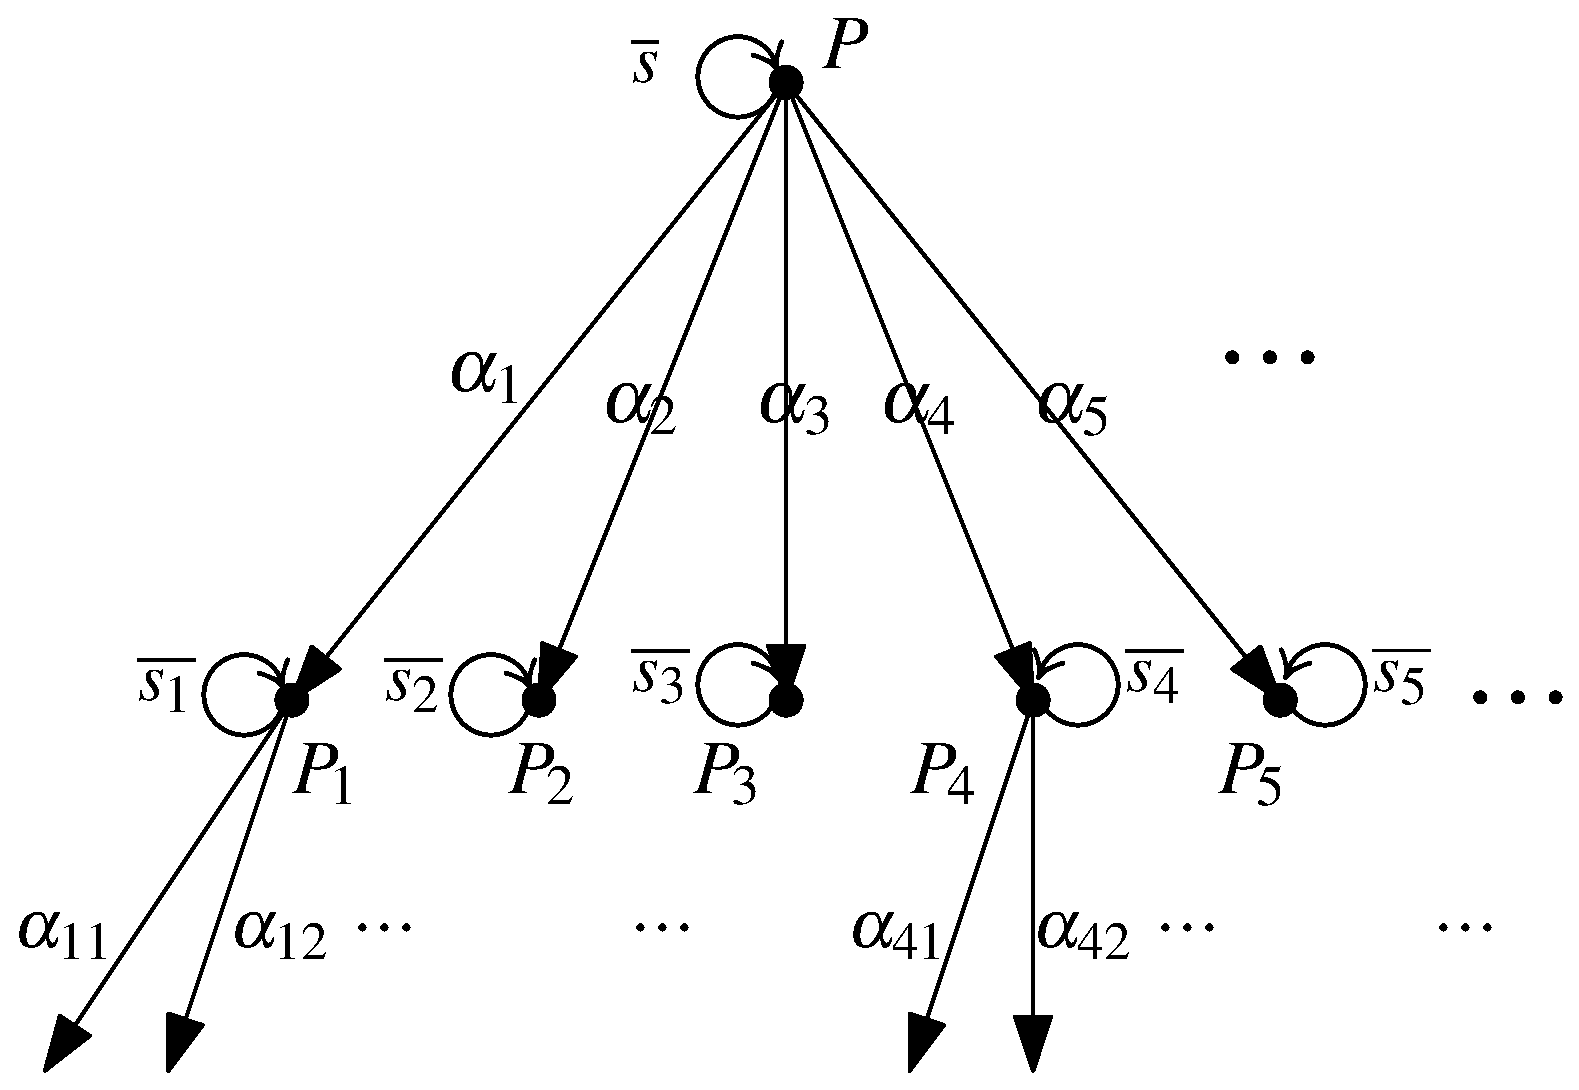
\includegraphics[width=0.5\textwidth]{images/semanticProof.eps}
  \end{figure}

  In conclusion, the process graphs of CCSS processes are also $\kappa$-bounded and can be expressed by CCS terms.
  To find such expressions, we first present the process graph of a certain CCSS process, then choose one of the CCS processes that expresses this process graph, this CCS process then also expresses the original CCSS process.

  This means that there exists an encoding from CCSS to CCS which satisfies all reasonable criteria (as mentioned in the proposition), but it is not compositional, as suggested by \pr{ccss-ccs-noncomp}.
\end{proof}

\begin{proposition}{ltsenc}
  The result in Proposition \ref{pr:ccss-ccs} extends to all process algebras that generate up to $\kappa$-bounded process graphs, including ABC and \CSG.
\end{proposition}

\begin{proof}
  Similar as the proof for \pr{ccss-ccs}.
\end{proof}

\subsection{CCSS to CCS, ABC, and \CSG}
\label{sec:ccss-ccs}

\begin{proposition}{ccss-ccs-noncomp}
  There is no compositional (\crt{comp}), divergence-reflecting (\crt{divref}) encoding from CCSS to CCS that preserves semantics (\crt{presem}) up to weak bisimulation (\df{wbisim}) or a finer (\df{finer}) equivalence relation.
\end{proposition}

Compositionality involves contexts, so the first step is to clarify the meaning of contexts.
Given a set of intended observables (barbs) $Obs\subseteq \Name\dcup\overline{\Name}$, \textbf{a context should not provide barbs / observables}.
If it does so, then every encoded term would for example exhibit barb $x\in Obs$, even $\bkt\nil$.
This would violate and nullify the meaning of barbs, which is to distinguish different processes by observing the barbs.
If every process exhibits the same barb, this barb then loses its purpose.

Also, \textbf{a context does not restrict barbs / observables}.
Again, if a context restricts $x\in Obs$, we cannot distinguish $\bkt{x}$ and $\bkt{\nil}$, which also contradicts with the purpose of barbs.

Finally, \textbf{a context does not depend on the process in its ``hole"}.
A context is fixed when the encoding is proposed, and requiring ``there is an $\alpha$ in $C$ if there is an $\alpha$ in $p$, and $\alpha$ becomes $\beta$ if $p$ has $\beta$ instead of $\alpha$", where $C$ is a context and $p$ is the process in its ``hole", means we require a ``variable" in the context, which does not exist in CCS and its extensions.

To prove the proposition, we first need to establish \lem{plustoplus}.

\begin{lemma}{plustoplus}
  %$\bkt{P+Q} = D(C_1(\bkt{P})+C_2(\bkt{Q}))$, where $C_1$, $C_2$, $D$ are contexts with one ``hole".
  The choice operator must be encoded into a choice operator in an encoding that is compositional, preserves divergence,  and preserves semantics up to weak bisimulation or a finer equivalence relation.
\end{lemma}

\begin{proof}
  Suppose the set of barbs include $\{y,z\}$.
  We first prove the lemma for weak bisimulation.
  For now $\eqv$ represents weak bisimulation.

  Consider the process $y+z\in\St_{CCSS}$.
  $\bkt{y+z} = C(\bkt y, \bkt z)$ where $C$ is a context (compositionality).
  Because $y+z$ is not divergent, $\bkt{y+z}$ is also not divergent (\lem{div}).
  Then there is a finite computation:
  \[\bkt{y+z} = C(\bkt y, \bkt z) \ar{} \ar{} \cdots \ar{} T \]
  where $T\nar{\tau}$.
  For all such computations, $\bkt{y+z}\vred{}T$ implies that $y+z\vred{} S$ where $S\eqv T$ by applying weak bisimilarity multiple times.
  Since $y+z$ does not reduce, we know that $y+z\vred{} S$ represents no transitions, and as a result $S=y+z$.
  $S\ar{y}$ and $S\eqv T$ implies that $T\vred{\hat{y}}$ (weak bisimulation).
  Because $T$ is the state we found on the computation that $T\nar{\tau}$, we know that $T\vred{\hat{y}}$ consists no $\tau$-transitions before $y$-transition and thus $T\ar{y}$, which means $T$ barbs $y$ directly.
  Analogously, $T\ar{z}$.

  As stated above, the context does not provide barbs.
  $T\ar y$ and $T\ar z$ at the same time implies that $T=D'(\bkt y, \bkt z)$ for some context $D'$.
  Otherwise, if $T$ contains only one of $\bkt y$ and $\bkt z$, $T\ar y {\wedge} T\ar z$ indicates that the context in $T$ provides $y$ or $z$, and this contradicts with the requirements on contexts.
  This in turn suggests that the computation $C(\bkt y, \bkt z) \ar{} \ar{} \cdots \ar{} T$ does not depend on the content in the ``holes", but merely on the context $C$, since $\bkt y$ and $\bkt z$ stay intact in $T$.

  \fig{ptt} shows the parse tree of process $T$ where each vertex represents an operator in CCS, the root is on top, and $\bkt y$, $\bkt{z}$ are each represented by a leaf.
  %The parse tree of $T$ is a subtree of the parse tree of $C(\bkt y, \bkt z)$, because $T$ is acquired by executing a sequence of silent actions from $C(\bkt y, \bkt z)$.
  \begin{figure}[ht]
    \caption{Parse Tree of $T$}
    \label{fig:ptt}
    \centering
    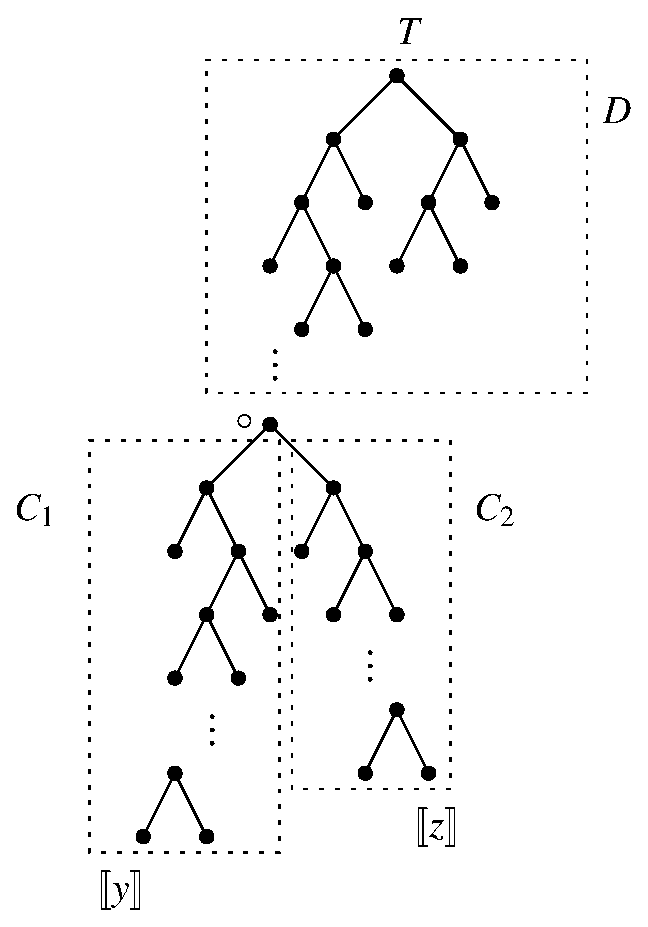
\includegraphics[width=0.35\textwidth]{images/ptt.eps}
  \end{figure}

  The circle $\circ$ in \fig{ptt} represents the first operator that connects the sub-tree including $\bkt y$ and $\bkt{z}$, that is, we can write $T = D(C_1(\bkt y)\circ C_2(\bkt{z}))$, where $D$ is the context with one ``hole" that is represented by \fig{ptt} excluding the sub-tree with $\circ$ as root,
  $C_1$ and $C_2$ are contexts with one ``hole" that is on the left / right side of $\circ$, respectively.

  This means that we can write $T=D(C_1(\bkt y)\circ C_2(\bkt z))$

  Considering $T\ar{y}\wedge T\ar z$, we know that no vertex in \fig{ptt} represents action prefixing, otherwise $T$ cannot barb $y$ and $z$ directly, i.e. $D$, $C_1$, $C_2$ contain no action prefixing.

\begin{comment}

$y+\tau.z\eqv \bkt{y+\tau.z}$ (preservation of semantics), and $y+\tau.z\ar{y}\nil$ implies $\bkt{y+\tau.z}\hvred{y}\eqv\nil$ (weak bisimulation).

Similarly, $\bkt{y+\tau.z}\hvred{\tau}R$, $R\eqv z$, which together with $z\ar{z}\nil$ imply $R\hvred{z} \eqv\nil$ (weak bisimulation).
We can compose the two paths together and acquire a new path (intermediate states are left out):
\[
\bkt{y+\tau.z} \hvred{\tau} \hvred{z} \eqv\nil
\]


  \begin{figure}[ht]
    \caption{Parse Tree of $\bkt{y+\tau.z}$}
    \label{fig:ptytauz}
    \centering
    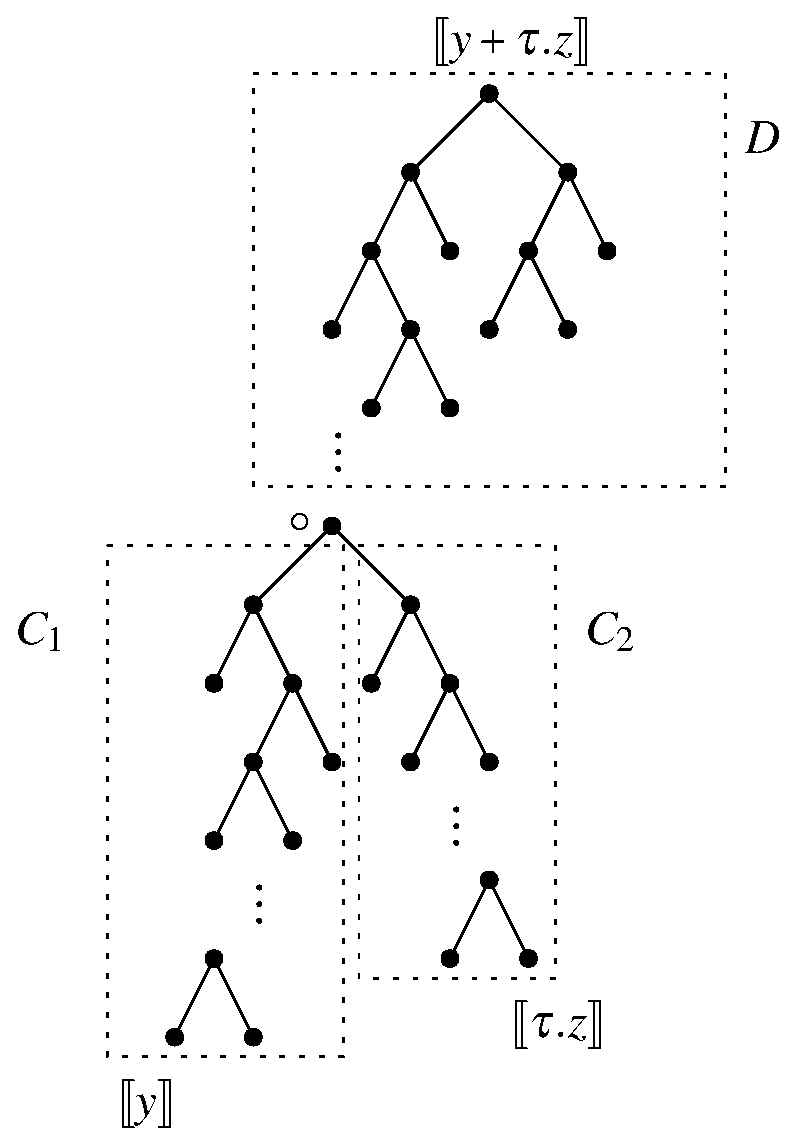
\includegraphics[width=0.35\textwidth]{images/ptytauz.eps}
  \end{figure}

\end{comment}

  Now consider the process $y+\tau.z\in\St_{CCSS}$.
  $\bkt{y+\tau.z} = C(\bkt y, \bkt{\tau.z})$ where $C$ is the same context as above.

  By applying weak bisimulation, the process graph of its encoding $\bkt{y+\tau.z}$ is in \fig{pgytauz} (dashed arrows represent transitions with a non-silent label, double lined arrow is as in \df{wbisim}).
  \begin{figure}[ht]
    \caption{Process Graph of $y+\tau.z$, $\bkt{y+\tau.z}$}
    \label{fig:pgytauz}
    \centering
    \includegraphics[width=0.4\textwidth]{images/pgytauz.eps}
  \end{figure}

  As mentioned before, the computation from $C(\bkt y, \bkt z)$ to $T=D(C_1(\bkt y)\circ C_2(\bkt z))$ only depends on $C$.
  Then $C(\bkt y, \bkt{\tau.z})$ can do a similar computation that only involves the context $C$ to $R=D(C_1(\bkt y)\circ C_2(\bkt{\tau.z}))$, where $D$, $C_1$, $C_2$ contain no action prefixing.

  Since $\tau.z\eqv\bkt{\tau.z}$ (preservation of semantics) and $\tau.z\ar{\tau}z$, we have $\bkt{\tau.z}\hvred{\tau}P$, $P\eqv z$, and subsequently $P\hvred{z} \eqv\nil$ (weak bisimulation).
  Analogously, $\bkt{y}\hvred{y} \eqv\nil$.

  Since the contexts $C_1$, $C_2$, $D$ contain no action prefixing, and they cannot restrict $y$, $z$, or $\tau$, we know that $C_1(\bkt y)$ can do $C_1(\bkt y)\hvred{y}$, where $C_1$ possibly contributes some $\tau$. ($P\hvred{\alpha}$ if and only if $\exists Q:\ P\hvred{\alpha}Q$.)

  Similarly, $C_2(\bkt{\tau.z})\hvred{\tau}\hvred{z}$.

  Suppose the operator $\circ$ is a parallel composition operator, then there is a path:
  \[C_1(\bkt y)\circ C_2(\bkt{\tau.z}) = C_1(\bkt y)|C_2(\bkt{\tau.z})\hvred{z}\hvred{y}\]
  because of \myref{par-l} and \myref{par-r}.
  The interleaving semantics of the parallel composition in CCS means that the process $P|Q$ can always execute any $\alpha$ if $P$ or $Q$ can execute $\alpha$.

  Because $D$ also does not restrict $y$, $z$, $\tau$, there is a path $R = D(C_1(\bkt y)|C_2(\bkt{\tau.z}))\hvred{z}\hvred{y}$.
  When we compose this path with the path from $\bkt{y+\tau.z}$ to $R$, we have a new path:
  \[\bkt{y+\tau.z}=C(\bkt y, \bkt z) \vred{} R \hvred{z} \hvred{y} \]
  This means that $\bkt{y+\tau.z}$ barbs both $y$ and $z$, which contradicts with the process graph of $\bkt{y+\tau.z}$ in \fig{pgytauz}.

  Since the other operators except for $+$ in CCS do not combine processes, the only possibility is that the $\circ$ is the choice operator $+$.

  Now suppose $\eqv'$ is an equivalence relation finer than weak bisimulation, then for all $P,\ Q\in\St_{CCSS}\cup\St_{CCS}$, $P\eqv Q$ implies $P\eqv' Q$, which means every implication in the above proof involving weak bisimulation is also true for $\eqv'$, and the lemma is also true for $\eqv'$.
\end{proof}


\begin{lemma}{paratopara}
  %$\bkt{P+Q} = D(C_1(\bkt{P})+C_2(\bkt{Q}))$, where $C_1$, $C_2$, $D$ are contexts with one ``hole".
  The parallel composition operator must be encoded into a parallel composition operator in an encoding that is compositional and preserves semantics up to weak bisimulation or a finer equivalence relation.
\end{lemma}

\begin{proof}
  The proof can be obtained by analysing the process $y|z$ in a way similarly as in the proof for \lem{plustoplus}.
\end{proof}

\begin{proof} (of \pr{ccss-ccs-noncomp})
  Consider the process $\nil\signals{s} + y$, with intended observables $\{y\}$, then $\bkt{\nil\signals{s} + y} = C(\bkt{\nil\signals{s}}, \bkt{y}))\vred{} V $ where $V = D(C_1(\bkt{\nil\signals{s}}) + C_2(\bkt{y}))$ with the same $C$, $D$, $C_1$, $C_2$ as in \lem{plustoplus}.
  %$V\eqv y$, since $\nil\signals{s} + y$ does not reduce.

  As mentioned earlier in the proof for \pr{ccss-ccs}, a process signalling $s$ can be treated as it doing an action $\overline{s}$ and returning back to itself.

  The process graphs are shown in \fig{pgsig} (by applying weak bisimulation).

  \begin{figure}[ht]
    \caption{Process Graphs of $\nil\signals{s} + y$ and $\bkt{\nil\signals{s} + y}$}
    \label{fig:pgsig}
    \centering
    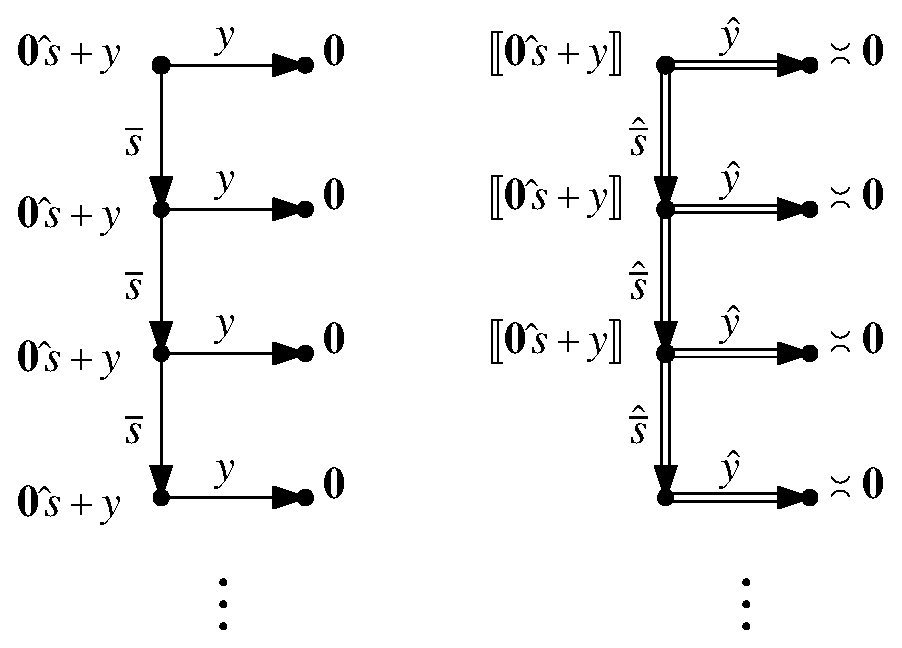
\includegraphics[width=0.4\textwidth]{images/pgsig.eps}
  \end{figure}

  Again by applying weak bisimulation, we can find a(n) (infinite) path $\bkt{\nil\signals{s}} \hvred{\overline{s}} \hvred{\overline{s}} \cdots$.

  Suppose either of $D$, $C_1$ restricts $s$, $V=D(C_1(\bkt{\nil\signals{s}})+C_2(\bkt{y}))$, would not be able to execute $s$ after a certain number of $\tau$ steps.
  At the same time, the context $C$ does not provide $s$, otherwise we would require $C$ to provide $r$ if we consider the process $\bkt{\nil\signals{r}+y}$, and this means the context $C$ depends on the process in its ``hole", which contradicts with the meaning of contexts.

  As a result, $\bkt{\nil\signals{r}+y}$ cannot weakly barb $s$, and this contradicts with the process graph of $\bkt{\nil\signals{s} + y}$ in \fig{pgsig}, and neither $D$ nor $C_1$ restricts $s$.

  Because $C_1$ and $C_2$ are connected with the choice operator, the process $C_1(\bkt{\nil\signals{s}})+C_2(\bkt y)$ has to choose between the lefthand and righthand side.
  Once a choice is made for $\overline{s}$, no more $y$ is possible, and vice versa.
  Hence there is no such path like \[C_1(\bkt{\nil\signals{s}})+C_2(\bkt y)\hvred{\overline{s}}\hvred{y}\cdots\] but only
  \[C_1(\bkt{\nil\signals{s}})+C_2(\bkt y)\hvred{\overline{s}}\hvred{\overline{s}}\cdots \text{, or }
  C_1(\bkt{\nil\signals{s}})+C_2(\bkt y)\hvred{y}\hvred{y}\cdots\].

  However, as shown in its process graph, $\bkt{\nil\signals{s} + y} $ has such path:
  \[
  \bkt{\nil\signals{s} + y} = C(\bkt{\nil\signals{s}}, \bkt{y})\hvred{\overline{s}}\hvred{y}\hvred{\overline{s}}\cdots
  \]
  which means that the context $C$ (or $D$) provides $\overline{s}$ after $C_1(\bkt{\nil\signals{s}})+C_2(\bkt{y})$ chooses $y$, and this contradicts with the requirements on contexts.
%  This means that the context $C'$ (or $D$) depends on the process in its ``hole", $C'$ (or $D$) changes if we put $C_1(\bkt{\nil\signals{r}}) + C_2{\bkt{y}}$ in its ``hole", and it violates the clarification at the beginning of this proposition.

  In conclusion, there is no path as
  \[\bkt{\nil\signals{s} + y} = C'(D(C_1(\bkt{\nil\signals{s}})+C_2(\bkt{y})))\hvred{\overline{s}}\hvred{y}\hvred{\overline{s}}\cdots\]
  and this contradicts with the process graph of $\bkt{\nil\signals{s} + y}$.

\end{proof}

Propositions \ref{pr:ccs-ccss} and \ref{pr:ccss-ccs-noncomp} together establish the fact that CCSS is strictly more expressive than CCS; CCSS is separated from CCS by compositionality.

\begin{proposition}{ccss-abc-noncomp}
  There is no compositional (\crt{comp}), divergence-reflecting (\crt{divref}) encoding from CCSS to ABC that preserves semantics (\crt{presem}) up to weak bisimulation (\df{wbisim}) or a finer equivalence relation.
\end{proposition}

\begin{proof}
  Again, the process $\bkt{y+\tau.z}$ can execute a series of reductions and reach a state $T'=D(C_1(\bkt y)\circ C_2(\bkt{\tau.z}))$ with the same contexts as before.

  Suppose the $\circ$ is parallel compositon.
  Because there is no action prefixing in either $C_1$ or $C_2$, the effect of broadcast mechanism has no effect on the proof.
  For example, even if there is such processes like $(b!|\bkt y) | \bkt{\tau.z}+b?$ or $(b! + \bkt y) | \bkt{\tau.z}+b?$, we can still find a path that includes $\hvred{z}\hvred{y}$, since the broadcast actions are not prefix of either $\bkt y$ or $\bkt{\tau.z}$.
  As a result, the $\circ$ must be a choice operator and the proof for \pr{ccss-ccs-noncomp} is still valid for ABC.
\end{proof}

\begin{proposition}{ccss-csg-noncomp}
  There is no compositional (\crt{comp}), divergence-reflecting (\crt{divref}) encoding from CCSS to \CSG that preserves semantics (\crt{presem}) up to weak bisimulation (\df{wbisim}) or a finer equivalence relation.
\end{proposition}

\begin{proof}
  In \CSG, only silent actions with higher priority can preempt the ecexution of other actions.
  Again, the process $\bkt{y+\tau.z}$ reduces to a state $T=D(C_1(\bkt y)\circ C_2(\bkt{\tau.z}))$ and there is no outgoing transitions labelled with any silent action.
  As a result, the priority mechanism plays no rule here.
  Suppose $\circ$ is a paralle composition, without any preemption, $C_1(\bkt y)$ and $C_2/\bkt{\tau.z}$ exhibiits interleaving semantics and we can find a path that includes $\hvred{z}\hvred{y}$.
  Again, by composing the two paths, we acquire a new path: $\bkt{y+\tau.z}\vred T \hvred{z}\hvred{y}$ and this leads to contradiction, and the choice operator must be encoded into a choice operator.

  The proof hereafter is identical with the proof for \pr{ccss-ccs-noncomp}.
  Note that the effect of priorities makes no distinction, because it only adds more conditions to the SOS-rules of the choice operator, but once a choice is made for the left hand side of $C_1(\bkt{\nil\signals s}) + C_2(\bkt y)$, it still becomes impossible to continue barbing $y$.
\end{proof}

In conclusion, CCSS cannot be compositionally encoded into CCS, ABC, \CSG up to a semantic-preserving encoding w.r.t. weak bisimulation or a finer relation.

\subsection{ABC to CCS and CCSS}
\label{sec:abc-ccs}
In \cite{PP16}, Pohjola and Parrow separated \emph{monotonic composition} and \emph{non-monotonic composition}.
In this \this, we use \emph{monotonic parallel composition} to separate ABC from CCS and CCSS.

\begin{definition}{monotonic}\textbf{(Monotonic Parallel Composition)}
  A parallel composition $| : \St\times\St\to\St$ is monotonic, if $\forall P, Q, R\in \St:\ P\vred{}Q$ implies $P|R\vred{}Q|R$.

  A parallel composition is \emph{non-monotonic}, if it is not monotonic.
\end{definition}
%Informally, monotonic compositions are the compositions that allow \emph{interleaving semantics}.

The parallel composition of CCS(S) is monotonic, which is easily derived from rules \myref{par-l} and \myref{par-r} in Table \ref{tab:CCSsos}.
In ABC it is not, due to the restriction in Table \ref{tab:ABCsos}, rules \myref{bro-l} and \myref{bro-r}.


\begin{proposition}{abc-ccs}
  \textbf{a)} There is no homomorphic (Criterion \ref{crt:homo}), divergence-reflecting (Criterion \ref{crt:divref}), and weakly observation-respecting (Criterion \ref{crt:obsres}.\ref{wobsres}) encoding from ABC to CCS;

  \textbf{b)} There is no homomorphic, barb preserving (\crt{bp}), and operational correspondent (Criterion \ref{crt:corr}) encoding from ABC to CCS, up to an equivalence that preserves barb (\df{bp}). % and is congruent (\df{cong}) w.r.t. parallel composition.


\end{proposition}

\begin{proof}
  By contradiction.

  \noindent\textbf{Part a)}: homomorphic, divergence-reflecting, and weakly observation-respecting.

  Reasonably, the intended observables are $Obs := \Act_{ABC}\backslash(\{\tau\}\cup\B!\cup\B?)$.
  Consider the process $P = (b! + b?).x + (d! + d?).y$, the process graph of P is shown in Figure \ref{fig:pgp} (note that the reduction relation is defined over $\{\tau\}\cup\B!$, dashed arrows represent non-reduction transitions):

  \begin{figure}[ht]
  \centering
  \caption{Process Graph of $P$}
  \label{fig:pgp}
  \vspace{3mm}
  \includegraphics[width = 0.27\textwidth]{images/pgp.eps}
  \end{figure}

  The process can make the choice between actions over channel $b$ or channel $d$, exposing $x$ or $y$, respectively.
  Once a choice is made between $b$ and $d$, either $x$ or $y$ is exposed, not at the same time.

  There are only two maximal computations of $P$:
  \[
    \pi_1: P\ar{}x;\
    \pi_2: P\ar{}y
  \]
  with $\Ob{\pi_1} = \{x\}$, $\Ob{\pi_2} = \{y\}$.
  Thus by Criterion \ref{crt:obsres}.\ref{wobsres} there exists maximal computations $\pi_1'$, $\pi_2'$ of $\bkt{P}$, such that $\Ob{\pi_1'} = \{x\} \wedge \Ob{\pi_2'} = \{y\}$.
  Suppose they are:
  \[
    \pi_1': \bkt{P}\red s_1 \red s_2 \red \cdots \red s_n;\
    \pi_2': \bkt{P}\red t_1 \red t_2 \red \cdots \red t_m
  \]
  We know that $\pi_1'$, $\pi_2'$ are finite because $\bkt{P}$ is not divergent ($P$ is not divergent, Lemma \ref{lem:div}).

  $\Ob{\pi_1'} = \{x\}$ means that $\exists s \in \{\bkt P, s_1, s_2, \dots s_n\}:s\ar{x}$ (\df{barb}).

  Similarly, $\exists t \in \{\bkt P, t_1, t_2, \dots t_m\}: t\ar{y}$.

  Now we look at the process $P|P$.
  Its process graph is shown in Figure \ref{fig:pgpp}:

  \begin{figure}[ht]
  \centering
  \caption{Process Graph of $P|P$}
  \label{fig:pgpp}
  \vspace{3mm}
  \includegraphics[width = 0.35\textwidth]{images/pgpp.eps}
  \end{figure}

  There are also only two maximal computations of $P|P$:
  \[
    \pi_3: P|P\red x|x;\
    \pi_4: P|P\red y|y
  \]
  with $\Ob{\pi_3} = \{x\} \wedge \Ob{\pi_4} = \{y\}$.

  The encoding of\ $P|P$\ however exhibits more barbs.
  $\bkt{P|P} = \bkt{P}|\bkt{P}$ (Criterion \ref{crt:homo}), and we can compose computations $\pi_1'$, $\pi_2'$ together and acquire a new computation:
  \[
    \pi_5:\bkt{P|P}=\bkt{P}|\bkt{P}\red s_1|\bkt P \red s_2|\bkt P \red \cdots \red s_n|\bkt{P}\red s_n|t_1 \red s_n|t_2 \red \cdots \red s_n|t_m
  \]

  For $P$, $Q$ $\in \St_{CCS}$, if $P\ar{x}$, then $P|Q\ar{x}$ and $Q|P\ar{x}$ (\mylabel{par-l}, \mylabel{par-r}).

  Thus $\exists s\in \{\bkt P|\bkt P, s_1|\bkt P, s_2|\bkt P, \dots s_n|\bkt P\}: s\ar{x}$ and $\exists t \in \{s_n|\bkt P, s_n|t_1, s_n|t_2, \dots s_n|t_m\}: t\ar{y}$, which means $\Ob{\pi_5} = \{x,y\}$, not a subset of either $\Ob{\pi_3}$ or $\Ob{\pi_4}$.
  $\lightning$ (\crt{obsres}.\ref{wobsres})

  \noindent\textbf{Part b)}: homomorphic, barb preserving, operational correspondent up to an barb preserving equivalence.
  %\begin{comment}
    %Too strong, but cannot prove it with weak barb preserving encoding.
  %\end{comment}

  Again consider the processes $P$ and $P|P$ with the set of observables that include $\{x, y\}$.

  $\bkt{P|P} = \bkt{P}|\bkt{P}$ (homomorphy).

  $P\vred{}x$ implies $\bkt{P}\vred{}S \wedge\, S\eqv \bkt{x}$ for some $S$ (completeness).
  Suppose the path is
  \[
    \pi_1 : \bkt{P}\ar{}\cdots\ar{} S
  \]

  $P\vred{}y$ implies $\bkt{P}\vred{}T$ where $T\eqv \bkt{y}$, with path
  \[
    \pi_2 : \bkt{P}\ar{}\cdots \ar{} T
  \]

  We can compose $\pi_1$ and $\pi_2$ into
  \[
    \pi_3 : \bkt{P|P} = \bkt{P}|\bkt{P}\ar{}\cdots\ar{} S|\bkt{P} \ar{}\cdots\ar{} S|T
  \]

  $x\barb x$ implies $\bkt x \barb_{\ren x}$ (barb preservation of $\enc$), thus $S \barb_{\ren x}$ (barb preservation of $\eqv$).
  Similarly, $T \barb_{\ren y}$.

  $\bkt x \barb_{\ren x}$ and $\bkt y \barb_{\ren y}$ implies $\bkt x|\bkt y \barb_{\ren x}$ and $S|T \barb_{\ren y}$:
  for all CCS (CCSS) processes $P$ and $Q$, if $P\barb x$ and $Q\barb y$, then $P\ar{x}$ and $Q\ar{y}$ (\df{barb}), then $P|Q\ar{x}$, $P|Q\ar{y}$, $Q|P\ar{x}$, and $Q|P\ar{y}$ (\myref{par-l}, \myref{par-r}),
  which means $P|Q\barb{x}$ and $P|Q\barb{y}$:

  In conclusion, $\bkt{P|P}\vred{}\eqv\bkt{x|y}$, and this implies $P|P\vred{} Q\wedge \bkt Q \eqv \bkt{x|y}$ for some $Q$ \myref{sound}, and $\bkt Q \barb_{\ren{x}} \wedge \bkt Q \barb_{\ren{y}}$ (barb preservation of $\eqv$).
  This in turn implies $Q\barb x \wedge Q \barb y$ (barb preservation of $\eqv$).

  This means that $P|P$ reduces to a state that barbs $x$ and $y$ at the same time, which contradicts the process graph of $P|P$. $\lightning$

\end{proof}


These separation results rely on the fact that broadcast actions enforce all the willing parts to participate, while the parallel composition operator in CCS allows the participants to act independently, a.k.a. the parallel operator is monotonic.
This result extends to CCSS, as CCSS also has monotonic parallel composition.

\begin{proposition}{abc-ccss}
  The separation results extends to CCSS.
\end{proposition}

\begin{proof}
  Same as \pr{abc-ccs} and ommited.
\end{proof}

\pr{abc-ccs} and \pr{abc-ccss} shows that ABC is separated from CCS and CCSS by homomorphy.

%\begin{proposition}{abc-ccs-comp}
%  There is (no) compositional encoding from ABC to CCS.
%\end{proposition}

%\begin{proof}

%\end{proof}
\begin{comment}
This might help prove abc-ccs:

  {\begin{corollary}{nred}
  If an encoding $\bkt{\cdot}$ respects \myref{Complete} creteria, then if $P$ does not reduce to a state that is not equivalent to $P$, then $\bkt{P}$ does not reduce to a state that is not equivalent to $\bkt{P}$. Formally:

  $P\nreduce_1 P'$ where $P'\neqv_1 P$, then $\bkt{P}\nreduce_2 T$ where $T\neqv_2 \bkt{P}$, if $\bkt{\cdot}$ respects \myref{Sound} criterion.
  \end{corollary}

  \begin{proof}
  ?
  \end{proof}
  }
\end{comment}



\subsection{ABC to \CSG}
\label{sec:abc-ccssg}
\begin{proposition}{abc-ccssg}
  There is a homomorphic (Criterion \ref{crt:homo}) encoding (w.r.t. all operators except prefixing for broadcast and receive actions) from ABC to \CSG (with 3 priorities) that respects operational correspondence (Criterion \ref{crt:corr}) up to identity function, and divergence reflection (Criterion \ref{crt:divref}).
\end{proposition}

%\input{proofABCsg.tex}
%%%%%%%%%%%%%%%%%%%%%%%%%%%%%%%%%%%%%%%%%%%%%%%%%%%%%%%%%%%%%begin proof
\begin{proof}
For readability, we write $\alpha_h$ for $\alpha\cln 0$, $\alpha_m$ for $\alpha\cln 1$, $\alpha_l$ for $\alpha\cln 2$, meaning high, medium, low priority, respectively.

The encoding $\enc$ is as follows\footnote{The encoding was originally proposed by Johannes \AA man Pohjola (Johannes.Amanpohjola@data61.csiro.au) during an afternoon tea session, and the proofs are done by the author.} ($b\in\B$, $\eta\in\HS_{ABC}\dcup\{\tau\}$):
\begin{center}
$\begin{array}{ll}
  \\ [2ex]
\end{array}$
$\begin{array}{lll}
  \bkt{b?.P} := b_h.\tau_m.\bkt{P} &
  \bkt{b!.P} := \tau_l.(\overline{b_h}.X + \tau_m.\bkt{P}) &
  \hspace{-2.5mm}\text{where }X \defis \overline{b_h}.X + \tau_m.\bkt{P}
  \\[1ex]
  \bkt{\eta.P} := \eta. \bkt{P} &
  \bkt{P | Q} := \bkt{P} | \bkt{Q} &
  \bkt{\sum_{i\in I}P_i} := \sum_{i\in I}\bkt{P_i}\ (I \text{ an index set})
  \\[1ex]
  \bkt{P[f]} := \bkt{P}[f'] &
  \bkt{P\backslash L} := \bkt{P} \backslash \ren{L} &
  \bkt{A} := P' \text{ for } A\defis P \text{, and } P'\defis\bkt{P}
  \\[1ex]
\end{array}$
\end{center}

The renaming policy
$\ren{x} :=
\begin{cases}
  x_h, \ \forall x\in\B\\
  x_l, \ \forall x \in \Name_{CCS}
\end{cases}$
is injective (please refer to \df{encd}), and it extends to $\Act_{ABC}$ by defining $\ren{\overline{x}}:=\overline{\ren{x}}$ ($x\in\Name_{CCS}$), $\ren{x?} := x_h$, $\ren{x!} := \overline{x_h}$ ($x\in\B$).
The extended renaming policy $\varphi_{\bkt{}}: \Act_{ABC}\to \Act_{ABC}$ is still injective.
Although both $x?$ and $x!$ are renamed to the same channel $x_h$, they are renamed into exclusively input or output actions, and this preserves the injectivity of the renaming policy.

The agent identifiers $X$ and $P'$ are \emph{fresh}, in the sense that every encoding of a process including broadcast action prefix  or agent identifier generates a different $X$ or $P'$, respectively.
For all $\alpha\in\Act_{ABC}$, the relabelling function $f'$ is defined as
$\begin{cases}
  f'(\alpha) := \alpha, & \text{ if } \alpha \notin image(\varphi_{\bkt{}}); \\
  f'(\ren{\alpha}) := \ren{f(\alpha)}, & \text{ else. }
\end{cases}$

$\ren{L}:=\{\ren{\alpha}\mid\alpha\in L\}$.
\\[1ex]
\indent$\bkt\nil = \bkt{\Sigma_{i\in\emptyset}P_i} = \Sigma_{i\in\emptyset}\bkt{P_i} = \nil$.

The encoding is homomorphic for all operators except prefixing with $b!$ and $b?$ per definition.
Its operational correspondence is established with Lemmas \ref{lem:direction1}, and \ref{lem:direction2}, and its divergence reflection is proved with \lem{divref}.

\end{proof}

\begin{lemma}{direction1}
  For all $S\in\St_{ABC}$, if $S \vred{} S'$ then $\bkt{S} \vred{} \bkt{S'}$.
  (The $\eqv$ symbol is left out because it is the identity function in this case, i.e. $P\eqv Q$ iff $P = Q$.)
\end{lemma}

\begin{proof}
  This lemma is trivially true if $S = S'$, because the relation $\vred{}$ is reflexive.
  If $S \neq S'$, we can write the path (computation) explicitly:
  \[
    S\ar{}s_1\ar{}s_2\ar{}\cdots s_{n-1}\ar{}S'
  \]
  for some $s_i\in\St_{ABC}$, $1\leq i\leq n-1$, $i\in \IN$.

  Applying Lemma \ref{lem:comp} $n$ times, there is a corresponding path in \CSG with 3 priorities:
  \[
    \bkt{S} \vred{} \bkt{s_1} \vred{} \bkt{s_2} \vred{} \cdots \bkt{s_{n-1}} \vred{} \bkt{S'}
  \]
  thus $\bkt{S} \vred{} \bkt{S'}$.
\end{proof}

\begin{lemma}{comp}
	For all $S \ar{} S'$, it holds that $\bkt{S} \vred{} \bkt{S'}$.
\end{lemma}

\begin{proof}
  If we explicitly label the transition as $S \ar{\alpha} S'$, then there are two possibilities (note in ABC the set of reduction labels is $\B!\dcup\{\tau\}$):

	\textbf{Case 1:} $\alpha=\tau$, this lemma is directly implied from Lemma \ref{lem:tau-comp}, whose proof is built upon Lemma \ref{lem:pree}, and \ref{lem:hc-comp}.

	\textbf{Case 2:} $\alpha \in \B!$, let $j=0$ in Lemma \ref{lem:bro-commu} then we have the proof. For Lemma \ref{lem:bro-commu} we need Lemma \ref{lem:bro-comp}.

\end{proof}

\begin{lemma}{pree}
	If $P$ is an ABC process, then $\nexists P',\ P'' \in \St_{CCS^{sg}}:\ \bkt{P}\ar{\tau_h} P' \vee \, \bkt{P}\ar{\tau_m} P''$, which means $\bkt{P}$ cannot preempt the execution of any action with priority $l$.
\end{lemma}
\begin{proof}
  By contradiction.
  Suppose $\bkt{P}$ can preempt the execution of some action, which means $\bkt{P}\ar{\tau_m}P'$ or $\bkt{P}\ar{\tau_h}P''$ for some $P',P''\in\St_{CCS^{sg}}$ (\df{pree}).

	From the encoding we can see: $\tau_m$ always has at least a $\tau_l$, $b_h$, or\ $\overline{b_h}$ as prefix, thus there is no outgoing transition labelled with $\tau_m$ from any $\bkt{P}$.

  Also, as shown in the encoding, there is no $\tau_h$ as subterm in $\bkt P$ for any $P$; there are only $b_h$ and $\overline{b_h}$ for some $b\in\B$ (please refer to Section \ref{sec:ccssg} for names in \CSG), which come from the encoding of $b?$ or $b!$, respectively.

  As a result, the transition $\bkt P\ar{\tau_h} S$ for some $S$ must involve the handshake communication of a pair of high-prioritised input and output actions.
  However, any $\overline{b_h}$ for $b\in\B$ has at least a $\tau_l$ as prefix, which means any transition involving $\overline{b_h}$ must follow (at least) one transition labelled with $\tau_l$.

  Thus any handshake communication resulting in $\tau_h$ must be a successor of (at least) one transition labelled with $\tau_l$, and there is no such transition: $\bkt P \ar{\tau_h}S$ for any $P\in\St_{ABC}$ and $S\in\St_{CCS^{sg}}$.

\end{proof}

\begin{lemma}{hc-comp}
	If $S$ is an ABC process, for all $S \ar{c} S'$ where $c \in \HS_{CCS}$, it holds that $\bkt{S}\ar{c_l}\bkt{S'}$.
\end{lemma}
\begin{proof}
	Trivially, the lemma holds for $S = \nil$.
  %Assume the lemma holds for some $P$, $Q$, $we prove by structural induction that it also holds for processes that are constructed using $P$, $Q$ and operators in ABC.
  Assume the lemma holds for some $P$, $Q$, $P_i$ ($i\in I$, $I$ an index set).
  We prove by structural induction that it also holds for processes that are constructed using $P$, $Q$, $P_i$ $(i\in I)$ and operators in ABC.

	\begin{itemize}
		\item \emph{Prefixing:} Suppose $S=c.P$, then $\bkt{S} = c_l.\bkt{P}$. $S\ar{c} S'\wedge S=c.P$ implies $S'=P$, and since $\bkt{S} = c_l.\bkt{P}$, we have $\bkt{S}\ar{c_l}\bkt P = \bkt{S'}$.
		\item \emph{Choice:} Suppose $S = \sum_{i\in I}P_i$, then $\bkt{S} = \sum_{i\in I}\bkt{P_i}$.
    Without loss of generality, we can assume $S \ar{c} S'$ derived from $P_j \ar{c} P'$ where $S' = P'$, $j\in I$.
    Since the lemma holds for $P_j$, we know that $\bkt{P_j}\ar{c_l}\bkt{P'}$, and thus $\bkt{S}\ar{c_l}\bkt{P'}=\bkt{S'}$.
		\item \emph{Parallel composition:} Suppose $S = P | Q$, $S \ar{c} S'$, then $\bkt{S} = \bkt{P}| \bkt{Q}$.
    Because $c \neq \tau$, the transition stems inevitably from either $P$ or $Q$.
		Suppose the transition stems from $P\ar{c}P'$, thus $S' = P'|Q$ and $\bkt{P}\ar{c_l}\bkt{P'}$.
    Now we can compose a path:
		\[ \bkt{S}= \bkt{P}|\bkt{Q}\ar{c_l}\bkt{P'}|\bkt{Q} =\bkt{S'} \]
    considering that $\bkt{Q}$ cannot preempt $c_l$ (Lemma \ref{lem:pree}).
    \item \emph{Agent Identifier:} Suppose $S\defis P$, then $S\ar{c}S'$ if and only if $P\ar{c}P'$ with $P'=S'$ (\myref{rec} in \tab{CCSsos}), which implies $\bkt{P}\ar{c_l}\bkt{P'}$.
    Since $\bkt{S} = P''$ where $P''\defis\bkt{P}$, we can infer $P''\ar{c_l}\bkt{P'}$ and thus $\bkt{S}\ar{c_l}\bkt{P'}=\bkt{S'}$ (SOS-rule for agent identifier in \tab{CCSsgsos}).
    \item \emph{Relabelling:} Suppose $S = P[f]$. $S\ar{c}S'$ implies $\exists a \in \Name_{ABC}:\ (f(a) = c) \wedge (P\ar{a}P') \wedge (S'=P'[f])$, otherwise the transition $S\ar{c}S'$ cannot be derived from any rule in Table \ref{tab:CCSsos}, which is a part of ABC semantics.
    The relabelling function in ABC is defined as $f:(\B\to\B)\cup(\Name_{CCS}\to\Name_{CCS})$ (Section \ref{sec:abc}), it maps handshake names to handshake names, thus $a\in\Name_{CCS}$ only when $c\in\Name_{CCS}$.
    Due to the induction hypothesis, $P\ar{c}P'$ implies $\bkt{P}\ar{a_l}\bkt{P'}$.

    $\bkt{S}=\bkt{P[f]}=\bkt{P}[f']$ and $\ren{f(a)}=f'(\ren{a})$.

    $\bkt{P}\ar{a_l}\bkt{P'}$ implies $\bkt{P}[f']\ar{f'(a_l)}\bkt{P'}[f']$ (Table \ref{tab:CCSsos} \myref{rel}), where $a_l$ is nothing special other than $\ren{a}$, and we might as well write it this way:

    \[
    f'(a_l) = f'(\ren{a}) \overset{\text{per definition}}{=} \ren{f(a)} \overset{\text{f(a)=c}}{=} \ren{c} = c_l.
    \]
    As a result, $\bkt{S}=\bkt{P[f]}=\bkt{P}[f']\ar{c_l}\bkt{P'}[f'] = \bkt{P'[f]} = \bkt{S'}$.

    \item \emph{Restriction:} Suppose $S=P\backslash L$, $S\ar{c}S'$ implies $P\ar{c}P',\ c, \overline{c}\notin L$ and $S'=P'\backslash L$, otherwise the transition $S\ar{c}S'$ cannot be derived from any rule in Table \ref{tab:CCSsos}.
    Thus $\bkt{P}\ar{c_l}\bkt{P'}$, where $c_l=\ren{c}$.

    $\ren{L}$ is defined as $\ren{L}:=\{\ren{\alpha}\mid\alpha\in L\}$.
    Because $\ren{}$ is injective, $c, \overline{c}\notin L$ implies $\ren{c}, \ren{\overline{c}}\notin\ren{L}$.
    Thus $\bkt{P}\ar{\ren{c}}\bkt{P'}$ implies $\bkt{P}\backslash \ren{L}\ar{\ren{c}}\bkt{P'}\backslash \ren{L}$, which is identical with $\bkt{P\backslash L}\ar{c_l}\bkt{P'\backslash L}$ and $\bkt{S}\ar{c_l}\bkt{S'}$.

    %TODO: the arrow crosses \ren .
	\end{itemize}
\end{proof}

\begin{lemma}{tau-comp}
	If $S$ is an ABC process, for all $S \ar{\tau} S'$, it holds that $\bkt{S}\ar{\tau_l}\bkt{S'}$.
\end{lemma}

\begin{proof}
  By structural induction.

  Replacing $c$ by $\tau$ in the proof for Lemma \ref{lem:hc-comp}, we have the proof for all cases except for transitions originated from handshake communication \myref{comm}: $S = P|Q \ar{\tau} S'$.
  We can assume without loss of generality that for some $c \in \HS_{CCS}$:
  \[
    S \ar{\tau} S'\text{ because }P \ar{c} P',\ Q \ar{\overline{c}} Q' \wedge S' = P'|Q'
  \]
  From Lemma \ref{lem:hc-comp} we know that $\bkt{P}\ar{c_l}\bkt{P'}$, $\bkt{Q}\ar{\overline{c_l}}\bkt{Q'}$.
  Because either the encoding of $P$ or $Q$ can preempt the execution of any action with priority $l$ (Lemma \ref{lem:pree}), $\bkt{P}$ and $\bkt{Q}$ can communicate on low-priority channel and form a silent action:
  \[
    \bkt{S} = \bkt{P}|\bkt{Q} \ar{\tau_l} \bkt{P'}|\bkt{Q'} = \bkt{S'}
  \]
\end{proof}

\begin{lemma}{notauh}
  For all $P\in\St_{CCS^{sg}}$, if $P\ar{\alpha_m}$ or $P\ar{\alpha_l}$ then $P\nar{\tau_h}$ for all $\alpha\in\Name_{CCS}$.
\end{lemma}

\begin{proof}
  First we need to prove that $P\ar{\tau_h}$ implies $\tau_h\in I(P)$.

  $P\ar{\tau_h}$ means that
  \begin{itemize}
    \item[i)] $\tau_h$ appears as subterm in $P$; (exclusive) or
    \item[ii)] there is at least a pair of $c_h$ and $\overline{c_h}$ in $P$ for some $c\in\Name_{CCS}$; (exclusive) or
    \item[iii)] both.
  \end{itemize}
   Otherwise we cannot find an SOS-rule in \tab{CCSsgsos} that results in a transition labelled with $\tau_h=\tau\cln 0$.

  As we can see from \tab{pias}, if $\alpha\cln k$ is a subterm of $P$, then it is always an element of $I(P)$ except when
  \begin{itemize}
    \item all occurrances of $\alpha\cln k$ are restricted in $P$, i.e. $\alpha\cln k$ is removed from $I(P)$ by set subtraction during the construction of $I(P)$; or
    \item all occurrances of $\alpha\cln k$ are renamed to some name other than itself.
  \end{itemize}

  However, when $\alpha\cln k = \tau_h = \tau\cln 0$, it can never be restricted, and it is always renamed to itself (please refer to \ref{sec:ccssg}).
  Therefore $\tau_h$ is always an element of $I(P)$ if it appears as a subterm in $P$, and this proves both i) and iii).

  In case of ii), since there is no $\tau_h$ as subterm in $P$, $P\ar{\tau_h}$ must stem from handshake communication, which means we must be able to find $P_1|P_2$ as subterm of $P$ that satisfies $P_1\ar{c_h}$ and $P_2\ar{\overline{c_h}}$ for some $c$.
  This implies that $c$ is not restricted in $P_1$ and $P_2$, and / or $c=f(a)$ for some $a$.

  Either way, $c\in I(P_1)$ and $\overline{c}\in I(P_2)$, which in turn implies that $\tau_h\in I(P_1|P_2)$, where $P_1|P_2$ is a subterm of $P$.

  With the same reasoning as before, $\tau_h$ cannot be restricted and is always renamed to itself, thus $\tau_h$ is an element of $I(P)$.

  Then we proceed to prove that ``$\forall \alpha_l, \alpha_m\in\Act_{CCS^{sg}}, P\in\St_{CCS^{sg}}$: if $P\ar{\alpha_l}$ or $P\ar{\alpha_m}$ then $P\nar{\tau_h}$", which is equivalent with ``$\forall \alpha_l, \alpha_m\in\Act_{CCS^{sg}}, P\in\St_{CCS^{sg}}$: if $P\ar{\tau_h}$ then $P\nar{\alpha}$ and $P\nar{\alpha_m}$".
%  Since $m=1$ and $l=2$, let $k$ range over $\{1,2\}$ then we can prove by induction:

  We can again prove it by structural induction.
  For instance, in case of parallel composition, if $P=P_1|P_2 \ar{\tau_h}$ stems from left interleaving, then $\tau_h = \tau\cln 0\in I(P_1)$.
  $I(P_1|P_2) = I(P_1) \cup I(P_2) \cup \{\tau\cln 0\mid I(P_1)\cap \overline{I(P_2)\neq \emptyset}\}$ (\tab{pias}), $I(P_1|P_2)$ is a superset of $I(P_1)$,
  which implies that $\tau_h\in I(P_1|P_2) = I(P)$, hence $P$ does not do any action with priority lower than $0$.
  The reasoning for other cases is similar and is omitted.

\end{proof}



\begin{lemma}{bro-comp}
	If $S$ is an ABC process, for all $S \ar{b?} S'$ where $b? \in \B?$, there exists $n \in \IN^+$ such that $\bkt{S}\ar{b_h}^n\ar{\tau_m}^n\bkt{S'}$, where $\ar{\alpha}^n$ is $n$ transitions sequentially composed: $\ar{\alpha}\ar{\alpha}\cdots\ar{\alpha}$.
\end{lemma}

\begin{proof}
  By structural induction.
	The lemma is again trivially true for $\nil$.
  Suppose it is also true for some $P, Q, P_i$ ($I$ an index set).

	\begin{itemize}
		\item \emph{Prefixing:} Suppose $S=b?.P$, there is only one outgoing transition from $S$ labelled with broadcast action: $S\ar{b?}P$, which means $S'=P$.
    $\bkt{S} = b_h.\tau_m.\bkt{P}$, there is a path: $\bkt S \ar{b?}\tau_m.\bkt P \ar{\tau_m} \bkt P =\bkt{S'}$.
    Let $n=1$ then the lemma is true.
    If $S=\alpha.P$ where $\alpha\notin\B?$ then there is no outgoing transition from $S$ with a receive label, the condition in the lemma does not hold, hence the lemma is true.
		\item \emph{Choice:} Similarly as in the proof for Lemma \ref{lem:hc-comp}.
		\item \emph{Parallel composition:} Suppose $S = P | Q$, $S \ar{b?} S'$, then $\bkt{S} = \bkt{P}| \bkt{Q}$.
		\begin{itemize}
			\item If the transition stems from interleaving (\myref{par-l}, \myref{par-r}, \myref{bro-l}, or \myref{bro-r}), we can again compose a path where $S' = P'|Q$ or $S'=P|Q'$ and prove the lemma, just as we did in the proof for Lemma \ref{lem:hc-comp}.
			\item If the transition stems from a broadcast-synchronisation (\myref{bro-c}), which means $S\ar{b?}S'$ stems from both $P\ar{b?}P'$ and $Q\ar{b?}Q'$, with $S'=P'|Q'$.
      Because the lemma is true for $P$ and $Q$ by induction hypothesis, there are two paths:
      \[
        \pi_1 : \bkt{P}\ar{b_h}^i R \ar{\tau_m}^i\bkt{P'}; \
        \pi_2 : \bkt{Q}\ar{b_h}^j T \ar{\tau_m}^j\bkt{Q'}.
      \]
      where $R$ and $T$ are intermediate states on $\pi_1$ and $\pi_2$.
      $R\ar{\tau_m}$ means $R\nar{\tau_h}$ (\lem{notauh}), and the same for $T$.
      This means that neither $R$ nor $S$ can preempt an action with medium priority.

      Now we can compose a third path:
      \[
        \pi_3 : \bkt{S}= \bkt{P}|\bkt{Q}\ar{b_h}^{i}R|\bkt{Q}\ar{b_h}^{j}R|T \ar{\tau_m}^{i}\ar{\tau_m}^{i} \bkt{P'}|\bkt{Q'}=\bkt{S'}
      \]
      Let $n = i + j$, the lemma is then also true for $S$.
      \item \emph{Agent Identifier:} Suppose $S\defis P$, the proof is similar to the proof for Lemma \ref{lem:hc-comp}.

      \item \emph{Relabelling:} Suppose $S = P[f]$, $S\ar{b?}S'$, then there exists $d$ such that $f(d)=b$ and $P\ar{d?}P'$ with $S'=P'[f]$, as stated in Lemma \ref{lem:hc-comp}.
      Thus $\bkt{P}\ar{d_h\,}^n\ar{\tau_m}^n\bkt{P'}$ for some $n$.
      Explicitly writing the path:
      \[
      \bkt{P}\ar{d_h\,}p_1\ar{d_h\,}\cdots\ar{d_h\,}p_n\ar{\tau_m}p_{n+1}\ar{\tau_m}\cdots\ar{\tau_m}p_{2n-1}\ar{\tau_m}\bkt{P'}
      \]
      Again, since $f'(d_h) = f'(\ren{d}) = \ren{f(d)} = \ren{b} = b_h$, and $f'(\tau_m) = \tau_m$ (considering $\tau_m$ is not in the image of $\ren{}$), we can apply Rule \myref{rel} $2n$ times and have the resulting path:
      \[
      \bkt{P}[f']\ar{b_h}p_1[f']\ar{b_h}\cdots\ar{b_h}p_n[f']\ar{\tau_m}p_{n+1}[f']\ar{\tau_m}\cdots\ar{\tau_m}p_{2n-1}[f']\ar{\tau_m}\bkt{P'}[f']
      \]

      Because $\bkt S = \bkt{P[f]}= \bkt{P}[f']$ and $\bkt{S'} = \bkt{P'[f]}= \bkt{P'}[f']$, we have the proof.

      \item \emph{Restriction:} Suppose $S=P\backslash L$, $S\ar{b?}S'$ implies $P\ar{b?}P'$ with $S'=P'\backslash L$ (broadcast names cannot be restricted).

      Again, $P\ar{b?}P'$ implies $\bkt{P}\ar{b_h}^n\ar{\tau_m}^n\bkt{P'}$.
      Since $b_h,\ \tau_m \notin \ren{L}$.
      Applying \myref{res} $2n$ times, we have a new path
      \[
      \bkt S = \bkt{P\backslash L}\bkt{P}\backslash\ren{L}\ar{b_h}^n
      \ar{\tau_m}^n\bkt{P'}\backslash\ren{L} = \bkt{P'\backslash L} = \bkt{S'}
      \]
      and we have the proof.
		\end{itemize}
	\end{itemize}
\end{proof}



\begin{lemma}{bro-commu}
	For all $j \in \IN$, if $P\ar{b!}P'$, then there exists $n \in \IN$ such that $ \bkt{P} \ar{\tau_l}\ar{\tau_h}^n\ar{\overline{b_h}}^j \ar{\tau_m}^{n+1} \bkt{P'}$.
\end{lemma}
Informally, this lemma states that the encoding translates one broadcast transition into a series of arbitrarily many $\overline{b_h}$ actions following and followed by a series of silent actions.
$n$ corresponds to the number of $b?$ that participated in the transition $P\ar{b!}P'$.

\begin{proof}
  The lemma is again trivially true for $\nil$.
  Suppose it is true for some processes $P$, $Q$, $P_i$ ($i\in I$, $I$ an index set), we prove it by structural induction.

	\begin{itemize}
		\item \emph{Prefixing:} Suppose $S = b!.P$, thus $\bkt{S} =  \tau_l.(\overline{b_h}.X + \tau_m.\bkt{P})$ where $X \defis \overline{b_h}.X + \tau_m.\bkt{P}$.
    After executing $\tau_l$, the $X$ provides an arbitrary number of $b_h$ actions, before executing a $\tau_m$ and reach the state $\bkt{P}$.
    Let $n = 0$, we have $S' = P'$ and the lemma is true for such $S$.
		\item \emph{Choice:} Same as in previous proofs.
		\item \emph{Parallel composition:} Suppose $S = P | Q$, $S \ar{b!} S'$, then $\bkt{S} = \bkt{P}| \bkt{Q}$.
	   	\begin{itemize}
	   		\item Suppose the transition stems from interleaving. The proof is again the same as in \lem{hc-comp}.
   			\item Suppose the transition stems from a broadcast communication, which means $P \ar{b!} P'$ and $Q \ar{b?} Q'$ or $P \ar{b?} P'$ and $Q \ar{b!} Q'$.
        Without loss of generality, we can assume it to be the first case.

        Lemma \ref{lem:bro-comp} implies that there exists $k > 0$ such that $\bkt{Q}\ar{b_h}^k T \ar{\tau_m}^k\bkt{Q'}$.
        Explicitly writing some of the intermediate states, we can construct the path
        \[
        \pi_1 : \bkt{Q}\ar{b_h}t_1\ar{b_h}\cdots\ar{b_h}t_k \ar{\tau_m}^k\bkt{Q'} \text{ (Lemma \ref{lem:bro-comp})}
        \]

        Since $\forall j \in \IN,\ \exists n \in \IN$ such that $ \bkt{P} \ar{\tau_l}\ar{\tau_h}^n\ar{\overline{b_h}}^j \ar{\tau_m}^{n+1} \bkt{P'}$ (induction hypothesis), it is also true for all $j$ not less than $k$: $0 < k \leq j$.
        Then we can find a path
   			\[
        \pi_2 : \bkt{P} \ar{\tau_l}\ar{\tau_h}^n r_0 \ar{\overline{b_h}} r_1 \ar{\overline{b_h}} \cdots \ar{\overline{b_h}} r_{k} \ar{\overline{b_h}} \cdots \ar{\overline{b_h}} r_j \ar{\tau_m}^{n+1} \bkt{P'}
        \]
        Composing the beginning of $\pi_2$ with a $\bkt Q$ to a new path ($\bkt{Q}$ cannot preempt any action)
        \[
        \pi_3 : \bkt{S}= \bkt{P}|\bkt{Q}\ar{\tau_l}\ar{\tau_h}^n r_0 | \bkt{Q}.
        \]
        Since $h$ is the highest priority level, the $b_h$ in $\pi_1$ and $\overline{b_h}$ in $\pi_2$ can always merge into a $\tau_h$ action; $t_k, t_{k+1}, \dots, \bkt{Q'}$ and $r_j, r_{j+1}, \dots, \bkt{P'}$ do not preempt $\tau_m$ (Lemmas \ref{lem:pree}, \ref{lem:notauh}).
        As a result, $\pi_3$ can be prolonged:
        \begin{align*}
          \pi_3' : \bkt{S}= \bkt{P}|\bkt{Q}
          & \ar{\tau_l}\ar{\tau_h}^n r_0 | \bkt{Q} \ar{\tau_h} r_1|t_1 \ar{\tau_h} r_2|t_2 \ar{\tau_h} \cdots \\
          & \ar{\tau_h} r_k|t_k \ar{\overline{b_h}} \cdots \ar{\overline{b_h}} r_j|t_k \ar{\tau_m}^{n+1}  \bkt{P'}|t_k \ar{\tau_m}^k \bkt{P'}|\bkt{Q'}
        \end{align*}
        $\pi_3'$ can be rewritten as
        \[
        \pi_3' : \bkt{S}= \bkt{P}|\bkt{Q} \ar{\tau_l}\ar{\tau_h}^{n+k} r_k|t_k \ar{\overline{b_h}}^{j-k} r_j|t_k \ar{\tau_m}^{n+1+k} \bkt{P'}|\bkt{Q'} = \bkt{S'}
        \]
        Let $j' = j - k$, we can always construct such $\pi_3'$ for all $k \leq j$ and thus for all $0 \leq j - k = j'$.
        Let $n' = n + k$, then we have found an $n'$ that makes the lemma true for transitions derivated from \myref{bro-comm}.
	   	\end{itemize}

    \item \emph{Agent Identifier:} Suppose $S\defis P$, the proof is again similar to that in Lemma \ref{lem:hc-comp}.

    \item \emph{Relabelling:} Suppose $S = P[f]$, then $\bkt{S} = \bkt{P}[f']$.
    $f'(\alpha) = \alpha$, if $\alpha \notin image(\varphi_{\bkt{}})$; $\ren{f(\alpha)}=f'(\ren{\alpha})$, else.

    $S\ar{b!}S'$, then there exists $d$ where $f(d) = b$, $P\ar{d!}P'$, and $S'=P'[f]$.
    The reason is the same as stated in Lemma \ref{lem:hc-comp}.

    Because $P\ar{d!}P'$, according to the induction hypothesis, it is true that for all $j \in \IN$, there exists $n \in \IN$ such that
    \[
    \bkt{P} \ar{\tau_l} \ar{\tau_h}^n\ar{\overline{d_h}\,}^j \ar{\tau_m}^{n+1} \bkt{P'}.
    \]
    Applying \myref{rel} $2(n+1)+j$ times, we have the path
    \[
    \bkt{P}[f'] \ar{f'(\tau_l)} \ar{f'(\tau_h)}^n\ar{f'(\overline{d_h\,})}^j \ar{f'(\tau_m)}^{n+1} \bkt{P'}[f'].
    \]
    where
    \begin{itemize}
      \item $f'(\tau_l) = f'(\ren{\tau}) = \ren{f(\tau)} = \ren{\tau} = \tau_l$;
      \item $f'(\tau_h) = \tau_h$, $f'(\tau_m) = \tau_m$ ($\tau_m$, $\tau_h$ not in the image of $\ren{}$);
      \item $f'(\overline{d_h}) = f'(\ren{d!}) = \ren{f(d!)} = \ren{b!} = \overline{b_h}$.
    \end{itemize}
    Replacing all the $f'(\cdot)$ in the path above, we have a new path:
    \[
    \bkt{P}[f'] = \bkt{P[f]} = \bkt{S} \ar{\tau_l} \ar{\tau_h}^n\ar{\overline{b_h\,}}^j \ar{\tau_m}^{n+1} \bkt{P'}[f'] = \bkt{P'[f]} = \bkt{S'}.
    \]

    \item \emph{Restriction:} Suppose $S=P\backslash L$, then $\bkt{S} = \bkt{P}\backslash \ren{L}$.
    $S\ar{b!}S'$ implies $P\ar{b!}P'$ with $S'=P\backslash L$.
    $b_h, \overline{b_h}, \tau_l, \tau_m, \tau_h \notin \ren{L}$ as before.

    As part of the induction hypothesis, it is true for all $j \in \IN$, there exists $n \in \IN$ such that
    \[
    \bkt{P} \ar{\tau_l} \ar{\tau_h}^n\ar{\overline{b_h}}^j \ar{\tau_m}^{n+1} \bkt{P'}.
    \]
    Apply \myref{res} $2(n+1)+j$ time, we have a new path
    \[
    \bkt{P}\backslash\ren{L} \ar{\tau_l} \ar{\tau_h}^n\ar{\overline{b_h}}^j \ar{\tau_m}^{n+1} \bkt{P'}\backslash\ren{L}.
    \]
    Since $\bkt S = \bkt{P \backslash L} = \bkt{P}\backslash\ren{L}$ and $\bkt{S'} = \bkt{P' \backslash L} = \bkt{P'}\backslash\ren{L}$ we have the proof.
	\end{itemize}
\end{proof}

%%%%%%%%%%%%%%%%%%%%%%%%%%%%%%%%%%%%%%%%%%%%%%%%%%%%%%%%%%%%%%%%%%%%%%%%%%%%%%%%%%%%%%%%%%%%%%%%%%%%%%%

\begin{lemma}{direction2}
  For all $S\in\St_{ABC}$, if $\bkt{S} \vred{} \bkt{S'}$ then $S \vred{} S'$.
\end{lemma}

\begin{proof}
  Again, because of reflexivity of $\vred{}$, the lemma is trivially true for $S=S'$, we only need to consider the case when $S$ is different from $S'$, which means the length of the computation $\bkt{S} \vred{} \bkt{S'}$ is greater than $0$.

  To begin with, we find the first state on the computation $\bkt{S} \vred{} \bkt{S'}$ that is equivalent to an encoding of some process $S_1\in\St_{ABC}$, and show that $S\vred{} S_1$.

  Formally, if $S$ is an ABC process, for all computations starting from $\bkt{S}$ such that for some $S'\in \St_{ABC}$,
  \[
  \bkt{S} \ar{} t_1 \ar{} t_2 \ar{} \cdots \ar{} t_n=\bkt{S'} \cdots
  \]
  and $\forall i < n$, $\nexists T \in \St_{ABC}: \ t_i = \bkt{T}$, then $S\ar{}S'$.

  We prove this statement by structural induction.
  Trivially, the statement is true for $\nil$.
  Suppose the statement is true for $P$, $Q$, $P_i$ ($i\in I$, $I$ an index set), and $S$ is a process built upon them.
  \begin{itemize}
    \item \emph{Prefixing:}
    \begin{itemize}
      \item If $S = b?.P$ or $S = c.P$ for some $b? \in \B?$, $c\in\HS_{CCS}$, then $\bkt{S} = b_h.\tau_m.\bkt P$ or $\bkt S = c_l.\bkt P$, respectively, and there is no computation with length greater than $0$ starting from $\bkt S$, since the only outgoing transition is not labelled with a reduction label, which means the condition does not hold and the implication is always true.
      \item If $S = \tau.P$, then $\bkt{S} = \tau_l.\bkt{P}$, which means $t_n = t_1 = \bkt{P}$, and $S\ar{}P=S'$, the statement holds.
      \item If $S = b!.P$, then $\bkt{S} = \tau_l.(\overline{b_h}.X + \tau_m.\bkt{P}),\ X \defis \overline{b_h}.X + \tau_m.\bkt{P}$.
      All possible computations with lengths greater than $0$ are
      \begin{itemize}
        \item $\bkt{S} \ar{\tau_l} X$; or
        \item $\bkt{S} \ar{\tau_l} X \ar{\tau_m} \bkt{P}$; or
        \item $\bkt{S} \ar{\tau_l} X \ar{\tau_m} \bkt{P} \cdots$
      \end{itemize}
      where $X$ is not an encoding of any ABC process, because $X\ar{\tau_m} \bkt{P}$, which means $X$ can preempt actions with low priority, and it contradicts with Lemma \ref{lem:pree}.
      Thus $t_n = t_2 = \bkt{P}$, and $S\ar{}P = S'$.
    \end{itemize}
    \item \emph{Choice:} Suppose $S = \sum_{i\in I} P_i$, then $\bkt S = \sum_{i\in I} \bkt{P_i}$.
    Without loss of generality, we can assume that the computation $\bkt S \vred{} \bkt{S'}$ derivated from $\bkt{P_j}\vred{}\bkt{S'}$ for some $j\in I$.
    As implied by induction hypothesis, $P_j\ar{} S'$, which in turn implies $S\ar{} S'$.
		\item \emph{Parallel composition:} Suppose $S = P|Q$, then $\bkt{S} = \bkt{P}|\bkt{Q}$.

    As suggested by \lem{pree}, any reduction with source state $\bkt S$ must be labelled with $\tau_l$.
    %And we can see from the encoding, if $\tau_l$ appears as a subterm of $\bkt S$, then it must be the encoding of a subterm $\tau$ of $S$, or appear as prefix of the encoding of some broadcast action in $S$.
    %As a result, $\bkt S \ar{\tau_l} s_1$ must originate either from the encoding of $\tau$, or the encoding of some broadcast action, or the encoding of some handshake actions that

    For a better analysis, we can \emph{decompose} the transition $\bkt S = \bkt P | \bkt Q \ar{\tau_l} s_1$ into two transitions.
    A \emph{decomposition} of a transition from a parallel composed process is the original transitions that led to this transition, following Tables \ref{tab:CCSsos}, \ref{tab:CCSSsos}, \ref{tab:ABCsos}, and \ref{tab:CCSsgsos}.

    For example, the transition $a|\overline{a}\ar{\tau}\nil|\nil$ can be decomposed to $a\ar{a}\nil;\ \overline{a}\ar{\overline{a}}\nil$.
    ($\alpha$ is short for $\alpha.\nil$.)

    For symmetry, we write the decomposition of $a|b\ar{a}\nil|b$ as $a\ar{a}\nil;\ b\ar{\nil}b$.
    There might be more than one decomposition for a transition.
    For instance, $X|Y\ar{\tau}X|Y$ where $X\defis\tau.X,\ Y\defis\tau.Y$ can be decomposed into $X\ar{\tau}X;\ Y\ar{\nil}Y$ or $X\ar{\nil}X;\ Y\ar{\tau}Y$.
    A decomposition of a path is defined in the obvious way.

    On the other hand however, there must be at least one decomposition, since the inference rules for transitions related to parallel composition in the aforementioned Tables all have a non-empty set of condition(s).

    The transition $\bkt S = \bkt P | \bkt Q \ar{\tau_l} s_1$ can be decomposed into:
    \begin{enumerate}[label=(\roman*)]
      \item \label{itm:one} $\bkt{P}\ar{\tau_l}p_1$; $\bkt{Q}\ar{\nil}q_1$.
      \item \label{itm:two} $\bkt{P}\ar{\nil}p_1$; $\bkt{Q}\ar{\tau_l}q_1$.
      \item \label{itm:three}$\bkt{P}\ar{c_l}p_1$; $\bkt{Q}\ar{\overline{c_l}}q_1$ for some $c\in\HS_{CCS}$.
    \end{enumerate}

    We can see from the encoding at the beginning of this subsection, the action $c_l$ only appears as the encoding of some handshake action $c$ in ABC, and an encoding of some ABC process always follows $c_l$, for any $c\in\HS_{ABC}$.
    Thus in case of \itm{three}, we know that $P\ar{c}P'$ with $p_1=\bkt{P'}$ for some $P'$, and $Q\ar{\overline{c}}Q'$ with $q_1=\bkt{Q'}$ for some $Q'$.

    Subsequently, $s_n=s_1=p_1|q_1=\bkt{P'}|\bkt{Q'}=\bkt{P'|Q'}$ for some $P'$, $Q'$.
    $P\ar{c}P'$ and $Q\ar{\overline{c}}Q'$ implies $S=P|Q\ar{\tau}P'|Q'$.

    We can see that cases \itm{one} and \itm{two} are symmetric, and the proof for one case also applies for the other case.
    Without loss of generality, we only prove case \itm{one}.

    When the transition $\bkt S \ar{\tau_l}s_1$ decomposes into \itm{one}, it stems either from handshake or silent action in $P$, or a broadcast action.
    If it stems from handshake communication in $P$, then $p_1$ is the encoding of some $P'$, since all $c_l\in\Act_{CCS^{sg}}$ are followed by the encoding of some ABC process.
    In this case, $\bkt S = \bkt P | \bkt Q \ar{\tau_l} p_1|\bkt Q = \bkt{P'}|\bkt Q = \bkt{P'|Q}$ and $S=P|Q\ar{\tau}P'|Q$ and we have the proof.

    If the transition above stemmed from a silent action of $P$, the proof is similar.

    If $\bkt S \ar{\tau_l}s_1$ stems from the encoding of a broadcast action, we know that $p_1$ is not an encoding of any ABC process, because $p_1$ has as subterm $\overline{b_h}.X+\tau_m.\bkt{P'}$ for some $b, P', X\defis \overline{b_h}.X+\tau_m.\bkt{P'}$ and $p_1\ar{\tau_m}$.

    Since $\bkt S \ar{\tau_l} s_1$ stems from a broadcast action, for $\bkt S$ to reduce to a state that is an encoding of some ABC process, the computation must be in such form:
    \[
      \bkt S \ar{\tau_l} s_1 \ar{\tau_h}^n s_{n+1} \ar{\tau_m}^{n+1} s_{2n+2} = \bkt{S'} \text{ where } s_1\ar{\overline{b_h}}
    \]
    for some $n\in\IN, b\in\B$ and $S'$.

    Intuitively, the first transition labelled with $\tau_l$ indicates the beginning of a broadcast communication, it enables $s_1$ with an outgoing transition labelled with $\overline{b_h}$ for some $b\in\B$, willing to engage in handshake communication with any $b_h$ in the system.
    If there is any $b_h$, it means that there were $b?$ in the source term $S$ willing to synchronise with $b!$.
    The $\overline{b_h}$ and $b_h$ communicate and form a transition $\tau_h$.
    The number of $\tau_h$ corresponds to the number of participating $b?$ in the source term, and the number of $\tau_m$ that followed $b_h$.

    After every $b_h$ is consumed, $\tau_m$ preempts all low-prioritised actions, which corresponds to handshake actions or the beginning of other broadcast actions in ABC.
    Only after all $\tau_m$ are executed, including the one in the encoding of $b!$, will the system reach a state where it is an encoding of some ABC process $S'$, which indicates the end of the broadcast communication, and the computation corresponds to a transition on a single broadcast channel ($b$) in the source term.
    Once a broadcast communication is initiated, which is indicated by the first $\tau_l$ in the computation, the system cannot engage in any other broadcast communication, since the encodings of all other $d!\in\B!$ in the system have a low-prioritised $\tau_l$ as prefix, and such $\tau_l$ is preempted by $\tau_h$ which results from the communication of $b_h$ and $\overline{b_h}$.

    In conclusion, the computation
    $\bkt S \ar{\tau_l} s_1 \ar{\tau_h}^n s_{n+1} \ar{\tau_m}^{n+1} s_{2n+2} = \bkt{S'}$ ($s_1\ar{\overline{b_h}}$)
    indicates that $S$ does a broadcast communication over channel $b$, and reach the state $S'$: $S\ar{b!}S'$.

    The formal proof of this statement consists of multiple inductions, it is tedious and omitted.

    Now we have discussed all possible situations, and the statement is therefore true when $S$ is the parallel composition of $P$ and $Q$.

    \item \emph{Agent Identifier:} Suppose $S\defis P$, then $\bkt S = P'$ where $P'\defis \bkt P$.
    $\bkt S\ar{}s_1\ar{}s_2\cdots\ar{}s_n=\bkt{S'}$ ($s_i$ is not an encoding of any ABC process, where $1\leq i < n$) indicates a path $P'\ar{}s_1\ar{}s_2\cdots\ar{}s_n=\bkt{S'}$ (\myref{res}),
    which implies the existence of the path $\bkt P \ar{}s_1\ar{}s_2\cdots\ar{}s_n=\bkt{S'}$, otherwise the transitions in the computation of $P'$ above cannot derive from any SOS-rule of \CSG.

    This computation of $\bkt P$ in turn implies that $P\ar{}S'$ (induction hypothesis), which means that $S\ar{}S'$ and we have the proof.

    \item \emph{Relabelling:} Suppose $S = P[f]$, then $\bkt{S} = \bkt{P[f]} = \bkt{P}[f']$.
    Any computation starting from $\bkt{P}$ where $p_n$ of all $p_i$ ($1\leq i\leq n$) is the only state that is an encoding of some ABC process $P'$:
    \[
    \bkt{P}\ar{\alpha_1}p_1\ar{\alpha_2}p_2\cdots\ar{\alpha_n}p_n\ (\alpha_i\in\{\tau_l,\,\tau_m,\,\tau_h\})
    \]
    implies a new computation by applying \myref{rel} $n$-times
    \[
    \bkt{P}[f']\ar{f'(\alpha_1)}p_1[f']\ar{f'(\alpha_2)}p_2[f']\cdots\ar{f'(\alpha_n)}p_n[f']
    \]
    which can be rewritten as
    \[
    \pi_3 : \bkt{P[f]}\ar{f'(\alpha_1)}p_1[f']\ar{f'(\alpha_2)}p_2[f']\cdots\ar{f'(\alpha_n)}p_n[f'] = \bkt{P'}[f'] = \bkt{P'[f]}
    \]
    where $P'[f] = S'$, $p_n[f']$ of all $p_i[f']$ ($1\leq i\leq n$) is the first state that is an encoding of some ABC process.

    We can prove by structural induction that $p_i[f']$ is the encoding of some $P\in\St_{ABC}$ implies $p_i$ is the encoding of some $Q\in\St_{ABC}$.
    The proof is not special and omitted.
    Intuitively, since any relabelling function does not change priority level, or relabels $\tau$, or turn output action into input action, the structure is preserved by applying the relabelling functions.
    The relabelling of low-prioritised names does not effect whether a \CSG process is an encoding of some ABC process, since any $\alpha_l$ ($\alpha\in\HS_{ABC}\dcup\{\tau\}$) itself is an encoding of $\alpha$, as shown in the encoding.
    The relabelling of broadcast names has no effect, either.
    If $p_i$ contains the encoding of some broadcast action, and we change the $b$ in $\tau_l.(\overline{b_h}.X + \tau_m.\bkt P)$ ($X\defis \overline{b_h}.X + \tau_m.\bkt P$) to any broadcast name, the resulting process is still an encoding of some ABC process.
    The same if $p_i$ conains the encoding of some receive action.

    As a result, $p_n[f']$ is the first state on the path such that it is an encoding of an ABC process.

    Because $P\ar{\alpha}P'$ where $\alpha\in\B\dcup\{\tau\}$ (induction hypothesis), by applying \myref{rel} we have $S=P[f]\ar{f(\alpha)}P'[f]=S'$, where $f(\alpha)\in\B\dcup\{\tau\}$ and we have the proof.

    \item \emph{Restriction:} Suppose $S=P\backslash L$, then $\bkt{S} = \bkt{P}\backslash \ren{L}$.
    Because broadcast and silent actions cannot be restricted, we can easily prove this statement with $S'=P'\backslash L$ for relevant $P'$.
  \end{itemize}


  Finally, we proceed to prove the lemma.
  If $\bkt{S}\vred{}\bkt{S'}$ by
    \[
      \bkt{S} \ar{} s_{11} \ar{} s_{12} \ar{} \cdots \ar{} \bkt{S_1} \ar{} s_{21} \cdots \ar{} \bkt{S_2} \ar{}s_{31} \cdots \ar{} \bkt{S_{k}} = \bkt{S'}
    \]
  where $s_{ij}$ is not the encoding of any ABC processes for all relevant $i$, $j$.
  Applying the result we obtained above $k$-times, we have $S\vred{}S_1\vred{}S_2\vred{}\cdots\vred{}S_k = S'$, and we have proven that if $\bkt{S}\vred{}\bkt{S'}$ then $S\vred{}S'$.
\end{proof}

\begin{lemma}{divref}
  If $\bkt{S}\divg$ then $S\divg$ for all $S\in\St_{ABC}$.
\end{lemma}

\begin{proof}
  By structural induction.
  $\bkt{\nil} = \nil$ is not divergent, thus the lemma is true for $\bkt\nil$.
\begin{itemize}
  \item \emph{Prefixing:} Suppose $S=\alpha.P$.
  \begin{itemize}
    \item if $\alpha\in\{\tau\}$, then $\bkt S = \tau_l.\bkt P$, and $\bkt S \divg$ if and only if $\bkt P \divg$, which implies $P\divg$ (induction hypothesis), and thus $S=\tau.P\divg$.
    \item if $\alpha\in\HS_{ABC}$, then there is no infinite computation from $S$, because $\alpha_l$ is not a reduction label.
    \item if $\alpha\in\B?$, then $\bkt S = b_h.\tau_m.\bkt P$, and the proof is same as the above case.
    \item if $\alpha\in\B!$, then $\bkt S = \tau_l.(\overline{b_h}.X+\tau_m.\bkt P)$, $X\defis\overline{b_h}.X+\tau_m.\bkt P$.
    The only infinite computation must include
    \[
      \bkt S \ar{\tau_l} X \ar{\tau_m} \bkt P \cdots
    \]
    thus $\bkt S \divg$ if and only if $\bkt P \divg$, and $P \divg$ implies $S \divg$.
  \end{itemize}

  \item \emph{Choice:} Suppose $S = \sum_{i\in I}P_i$, the proof is straightforward.

  \item \emph{Parallel composition:} Suppose $S = P|Q$, then $\bkt{S} = \bkt{P}|\bkt{Q}$.
  When we decompose the infinite computation starting from $\bkt S$, each transition is decomposed either into a silent action of $\bkt P$ ($\bkt Q$) and no action of $\bkt Q$ ($\bkt P$), or a handshake communication between $\bkt P$ and $\bkt Q$.
  Either way, for $\bkt S$ to diverge, either $\bkt P$ or $\bkt Q$ or both are divergent, which implies $P$ or $Q$ or both are divergent.
  Since there is no preepmtion mechanism in ABC, $S=P|Q$ is also divergent.

  \item \emph{Agent Identifier:} Suppose $S\defis P$, then $\bkt S = P'$ where $P'\defis \bkt P$.

  $\bkt S \divg$ means that there is an infinite path
  \[
    \pi_1 : \bkt S = P' \ar{\alpha_1} s_1 \ar{\alpha_2} s_2 \ar{\alpha_3} s_3 \ar{} \cdots
  \]
  where $\alpha_i$ is silent action for all relevant $i$.

  Since $P'\defis \bkt P$, there must also be an infinite path
  \[
    \pi_2 : \bkt P \ar{\alpha_1} p_1 \ar{\alpha_2} p_2 \ar{\alpha_3} p_3 \ar{} \cdots
  \]
  otherwise the transitions in $\pi_1$ cannot be derived from any SOS-rules of \CSG.
  This means that $\bkt P\divg$, which in turn implies $P\divg$ and thus by applying the SOS-rule for agent identifier in \tab{CCSsgsos} we acquire an infinite computation with $S$ as the source state, i.e. $S\divg$.

  \item \emph{Relabelling:} Suppose $S = P[f]$, then $\bkt{S} = \bkt{P[f]} = \bkt{P}[f']$.
  $\bkt S \divg$ means that there is an infinite path:
  \[
  \pi_1 : \bkt S = \bkt{P}[f'] \ar{\alpha_1} s_1 \ar{\alpha_2} s_2 \ar{\alpha_3} s_3 \ar{\alpha_4} \cdots
  \]
  where $\alpha_i\in\{\tau_l, \tau_m, \tau_h\}$ for all relevant $i$.

  Since renaming functions do not map silent actions to non-silent actions, and they do not change priority levels, we always have $f(\tau_i) = \tau_i$ where $i=h$, $i=m$, or $i=l$ for any renaming function $f$.
  This means that the existence of $\pi_1$ implies the existence of $\pi_2$:
  \[
  \pi_2 : \bkt{P} \ar{\alpha_1} p_1 \ar{\alpha_2} p_2 \ar{\alpha_3} p_3 \ar{\alpha_4} \cdots
  \]
  where $\alpha_i\in\{\tau_l, \tau_m, \tau_h\}$ and $s_i=p_i[f']$ for all relevant $i$.
  This means that $\bkt S\divg$ implies $\bkt P\divg$ which in turn implies $P\divg$ (induction hypothesis).

  Because $S=P[f]$, $f$ maps silent action to silent action, $P\divg$ implies $S=P[f]\divg$.

  \item \emph{Restriction:} Suppose $S=P\backslash L$, then $\bkt{S} = \bkt{P}\backslash \ren{L}$.
  $\bkt{S} = \bkt{P}\backslash \ren{L}$ is divergent implies $\bkt P$ is divergent, thus $P$ is divergent and $S=P\backslash L$ is divergent, because silent actions cannot be elements of $L$.
\end{itemize}
\end{proof}

Now we have proved operational completeness with \lem{direction1}, and operational soundness with \lem{direction2}.
Divergence reflection is proved in \lem{divref}.
In conclusion, the encoding proposed at the beginning of this subsection is valid up to the aforementioned criteria.



\subsection{\CSG to CCS, CCSS, and ABC}
\label{sec:ccssg-ccs}
In their paper, Versari, Busi and Gorrieri separated \CSG from $\pi$-Calculus as well as $b\pi$-Calculus \cite{VBG09}.
We show in the following propositions that the same result extends to CCS, CCSS, and ABC.

\begin{proposition}{csg-abc}
  There is no homomorphic (\crt{homo}), weakly-observation-respecting (\ref{crt:obsres}.\ref{wobsres}) encoding from \CSG to ABC.
\end{proposition}

\begin{proof}
  Consider the process $P$ with the set of ovservables $Obs=\{n_l,y_l\}$, where
  \[
  P = \overline{m_l} \mid \overline{s_h} \mid \overline{q_h} \mid k_h. (s_h|q_h|\overline{k_h}) \mid m_l.s_h. (s_h.q_h. (\overline{k_h}|n_l) \mid \overline{r_l} \mid r_l.q_h.y_l)
  \ \footnote{In their original paper, Versari, Busi and Gorrieri studied a simpler variation of \CSG with slightly different syntax than in this \this.
  We changed the representation so it is uniform with other sections of this \this, but the process itself is essentially the same. }
  \]
  There are only two priority levels considered here.
  $h=0$ stands for high priority, $l=1$ stands for low priority.

  There is only one maximal computation of $P$, where the reductions originated from the handshake communication over $m_l$, $s_h$, $r_l$, $q_h$, consecutively.
  The subterms that form the next reduction are highlighted in bold, and we write $P$ instead of $P|\nil$ for readability:
  \begin{align*}
    \C_1 :
    & \mathbf{\overline{m_l}} \mid \overline{s_h} \mid \overline{q_h} \mid k_h. (s_h|q_h|\overline{k_h}) \mid \mathbf{m_l}.s_h. (s_h.q_h. (\overline{k_h}|n_l) \mid \overline{r_l} \mid r_l.q_h.y_l) \\
    \ar{\tau_l} & \mathbf{\overline{s_h}} \mid \overline{q_h} \mid k_h. (s_h|q_h|\overline{k_h}) \mid \mathbf{s_h}. (s_h.q_h. (\overline{k_h}|n_l) \mid \overline{r_l} \mid r_l.q_h.y_l) \\
    \ar{\tau_h} & \overline{q_h} \mid k_h. (s_h|q_h|\overline{k_h}) \mid s_h.q_h. (\overline{k_h}|n_l) \mid \mathbf{\overline{r_l}} \mid \mathbf{r_l}.q_h.y_l \\
    \ar{\tau_l} & \mathbf{\overline{q_h}} \mid k_h. (s_h|q_h|\overline{k_h}) \mid s_h.q_h. (\overline{k_h}|n_l) \mid \mathbf{q_h}.y_l \\
    \ar{\tau_h} & k_h. (s_h|q_h|\overline{k_h}) \mid s_h.q_h. (\overline{k_h}|n_l) \mid y_l
  \end{align*}
  where $\Ob{\C_1} = \{y_l\}$.

  The process $P|P$ has different computations, one of which is:
  \begin{align*}
    \C_2 :
    & P|P \ar{\tau_l} \ar{\tau_h} \text{ (handshake communication over $m_l$ and $s_h$)} \\
    & \overline{q_h} \mid k_h. (s_h|q_h|\overline{k_h}) \mid \mathbf{s_h}.q_h. (\overline{k_h}|n_l) \mid \overline{r_l} \mid r_l.q_h.y_l \mid \\
    & \overline{m_l} \mid \mathbf{\overline{s_h}} \mid \overline{q_h} \mid k_h. (s_h|q_h|\overline{k_h}) \mid m_l.s_h. (s_h.q_h. (\overline{k_h}|n_l) \mid \overline{r_l} \mid r_l.q_h.y_l) \\
    \ar{\tau_h}
    & \overline{q_h} \mid k_h. (s_h|q_h|\overline{k_h}) \mid \mathbf{q_h}. (\overline{k_h}|n_l) \mid \overline{r_l} \mid r_l.q_h.y_l \mid \\
    & \overline{m_l} \mid \mathbf{\overline{q_h}} \mid k_h. (s_h|q_h|\overline{k_h}) \mid m_l.s_h. (s_h.q_h. (\overline{k_h}|n_l) \mid \overline{r_l} \mid r_l.q_h.y_l) \\
    \ar{\tau_h}
    & \overline{q_h} \mid \mathbf{k_h}. (s_h|q_h|\overline{k_h}) \mid \mathbf{\overline{k_h}} \mid n_l \mid \overline{r_l} \mid r_l.q_h.y_l \mid \\
    & \overline{m_l} \mid k_h. (s_h|q_h|\overline{k_h}) \mid m_l.s_h. (s_h.q_h. (\overline{k_h}|n_l) \mid \overline{r_l} \mid r_l.q_h.y_l) \\
    \ar{\tau_h}
    & \overline{q_h} \mid s_h \mid q_h \mid \mathbf{\overline{k_h}} \mid n_l \mid \overline{r_l} \mid r_l.q_h.y_l \mid \\
    & \overline{m_l} \mid \mathbf{k_h}. (s_h|q_h|\overline{k_h}) \mid m_l.s_h. (s_h.q_h. (\overline{k_h}|n_l) \mid \overline{r_l} \mid r_l.q_h.y_l) \\
    \ar{\tau_h}
    & \mathbf{\overline{q_h}} \mid s_h \mid q_h \mid n_l \mid \overline{r_l} \mid r_l.q_h.y_l \mid \\
    & \overline{m_l} \mid s_h \mid \mathbf{q_h} \mid \overline{k_h} \mid m_l.s_h. (s_h.q_h. (\overline{k_h}|n_l) \mid \overline{r_l} \mid r_l.q_h.y_l) \\
    \ar{\tau_h}
    & s_h \mid q_h \mid n_l \mid \overline{r_l} \mid r_l.q_h.y_l \mid \\
    & \overline{m_l} \mid s_h \mid \overline{k_h} \mid m_l.s_h. (s_h.q_h. (\overline{k_h}|n_l) \mid \overline{r_l} \mid r_l.q_h.y_l) \\
    & = Q
    \end{align*}
    and $n_l\in\Ob{\C_2}$.

    When the computation reaches state $Q$, there is no more $\overline{q_h}$ in $Q$, which means that $q_h$ in $Q$ will never participate in a handshake communication, hence any computation of $Q$ will never exhibit the observable $y_l$, since all $y_l$ in $Q$ have $q_h$ as prefix.

    When we list all maximal computations of $P|P$, they all inevitably has $Q$ or a state that is structurally congruent (\tab{syneq}) with $Q$ as an intermediate state.
    This means that for all maximal computations $\C_i$ of $P|P$, it holds that $\Ob{\C_i}=\{n_l\}$ and $y_l\notin \Ob{\C_i}$.

    Suppose there is a homomorphic encoding from \CSG to ABC that is weakly observation-respecting, then the existence of the maximal computation $\C_1$ of $P$ implies the existence of a maximal computation $\C_1'$ of $\bkt{P}$ that satisfies $\Ob{\C_1'} = \Ob{\C_1} = \{y_l\}$ (weak observation-respecting encoding).

    This together with $\bkt{P|P} = \bkt{P}|\bkt{P}$ (homomorphy) implies that there exists a maximal computation $\C_1''$ of $\bkt{P}|\bkt{P}$ such that $\Ob{\C_1'} = \{y_l\}\subseteq \Ob{\C_1''}$ (\lem{paraabcmax}).

    This contradicts with the result obtained above that no maximal computation of $\bkt{P}|\bkt{P}$ exhibits $y_l$.
\end{proof}

\begin{lemma}{paraabc}
  Given a set of observables $Obs\subseteq\HS_{ABC}$, for all $P$, $Q\in\St_{ABC}$, if $P$ has a computation $\C$, then there exists a computation $\C'$ of $P|Q$ such that $\Ob{\C}\subseteq\Ob{\C'}$.
\end{lemma}

\begin{proof}
  Suppose $\C$ is a (possibly infinite) computation of $P$.
  If $\C$ contains no reduction, then $\Ob{\C} = \Ob{P}$ (\df{barb}), then there is a computation $\C'$ of $P|Q$ with no reduction and $\Ob{\C'} = \Ob{P|Q}$.

  For all $S$, $T\in\St_{ABC}$ and $x\in Obs \subseteq \HS_{ABC}$, $S\barb x$ implies $S|T \barb x$ (please refer to SOS-rules for ABC in Section \ref{sec:abc}), which means that $\Ob{S}\subseteq \Ob{S|T}$.
  As a result, $\Ob{\C} = \Ob{P}\subseteq \Ob{P|Q} = \Ob{\C'}$.

  If $\C$ contains at least one reduction, then we can write the (possibly infinite) computation $\C$ explicitly:
  \[
  \C : p_0\ar{\alpha_1}p_1\ar{\alpha_2}p_2\ar{\alpha_3}\cdots\ar{}p_n\cdots
  \]
  where $p_0 = P$ and $\alpha_i\in\{\tau\}\cup\B!$, $0\leq i$.

  If $\alpha_1 = \tau$, then by applying \myref{par-l} in \tab{CCSsos}, we acquire a reduction $P|Q = p_0|Q \ar{\alpha_1}p_1|q_1$ where $q_1=Q$;
  if $\alpha_1 = b!$ for some $b \in \B$, then by applying \myref{bro-l} (if $Q\nar{b?}$) or \myref{bro-c} (if $Q\ar{b?}Q'$) in \tab{ABCsos}, we again acquire a computation $P|Q\ar{\alpha_1}p_1|q_1$ where $q_1=Q$ or $q_1=Q'$, respectively.

  We can do the same for all $\alpha_i$ and acquire a computation $\C'$:
  \[
  \C' : p_0|q_0\ar{\alpha_1}p_1|q_1\ar{\alpha_2}p_2|q_2\ar{\alpha_3}\cdots\ar{}p_n|q_n\cdots
  \]
  where $p_0 = P$, $q_0 = Q$.

  The sets of observables satisfy $\Ob{\C} = \{x \mid \exists p_i: p_i\barb x (i\in\IN)\}$ and $\Ob{\C'} = \{x \mid \exists p_i|q_i: p_i|q_i\barb x (i\in\IN)\}$ (\df{barb}).
  If $x\in\Ob{\C}$, then there exists $p_i$ such that $p_i\barb x$ and thus $p_i|T\barb x$ for all $T$.
  This in turn implies that there exists $p_i|q_i$ such that $p_i|q_i\barb x$, and hence $x\in\Ob{\C'}$, which implies $\Ob{\C}\subseteq \Ob{\C'}$.

  The existence of $\C'$ proves the lemma.
\end{proof}

\begin{lemma}{paraabcmax}
  Given a set of observables $Obs\subseteq\HS_{ABC}$, for all $P$, $Q\in\St_{ABC}$, if $P$ has a \underline{maximal} computation $\C$, then there exists a \underline{maximal} computation $\C'$ of $P|Q$ such that $\Ob{\C}\subseteq\Ob{\C'}$.
\end{lemma}

\begin{proof}
  If $\C$ is a maximal computation of $P$, then by definition, $\C$ is also a computation, which implies that there exists a computation $\C'$ of $P|Q$ such that $\Ob{\C}\subseteq\Ob{\C'}$ (\lem{paraabc}).

  If $\C'$ is maximal, the lemma is true.
  If $\C'$ is not maximal, then we can extend $\C'$ to a maximal computation $\C''$.
  From the definition of $Obs$ we can see that $\Ob{\C'}\subseteq \Ob{\C''}$, and thus $\Ob{\C}\subseteq \Ob{\C''}$.
\end{proof}

\begin{proposition}{csg-ccs-s}
  There is no homomorphic (\crt{homo}), weakly-observation-respecting (\ref{crt:obsres}.\ref{wobsres}) encoding from \CSG to CCS or CCSS.
\end{proposition}

\begin{proof}
  \lem{paraabcmax} stays true if we replace ABC by CCS or CCSS (\myref{par-l}, \myref{par-r} in \tab{CCSsos}), and with the same reasoning as in the proof for \pr{csg-abc}, we can prove this proposition.
\end{proof}

\section{Conclusion}
\label{sec:conclusion}
The graph in \fig{map} shows the main results of this \this: encodability relations between CCS, CCSS, ABC, and \CSG.
Each arrow represents an encodability or separation result.

\begin{figure}[ht]
  \centering
  \caption{Encodability Relations Between CCS, CCSS, ABC, and \CSG}
  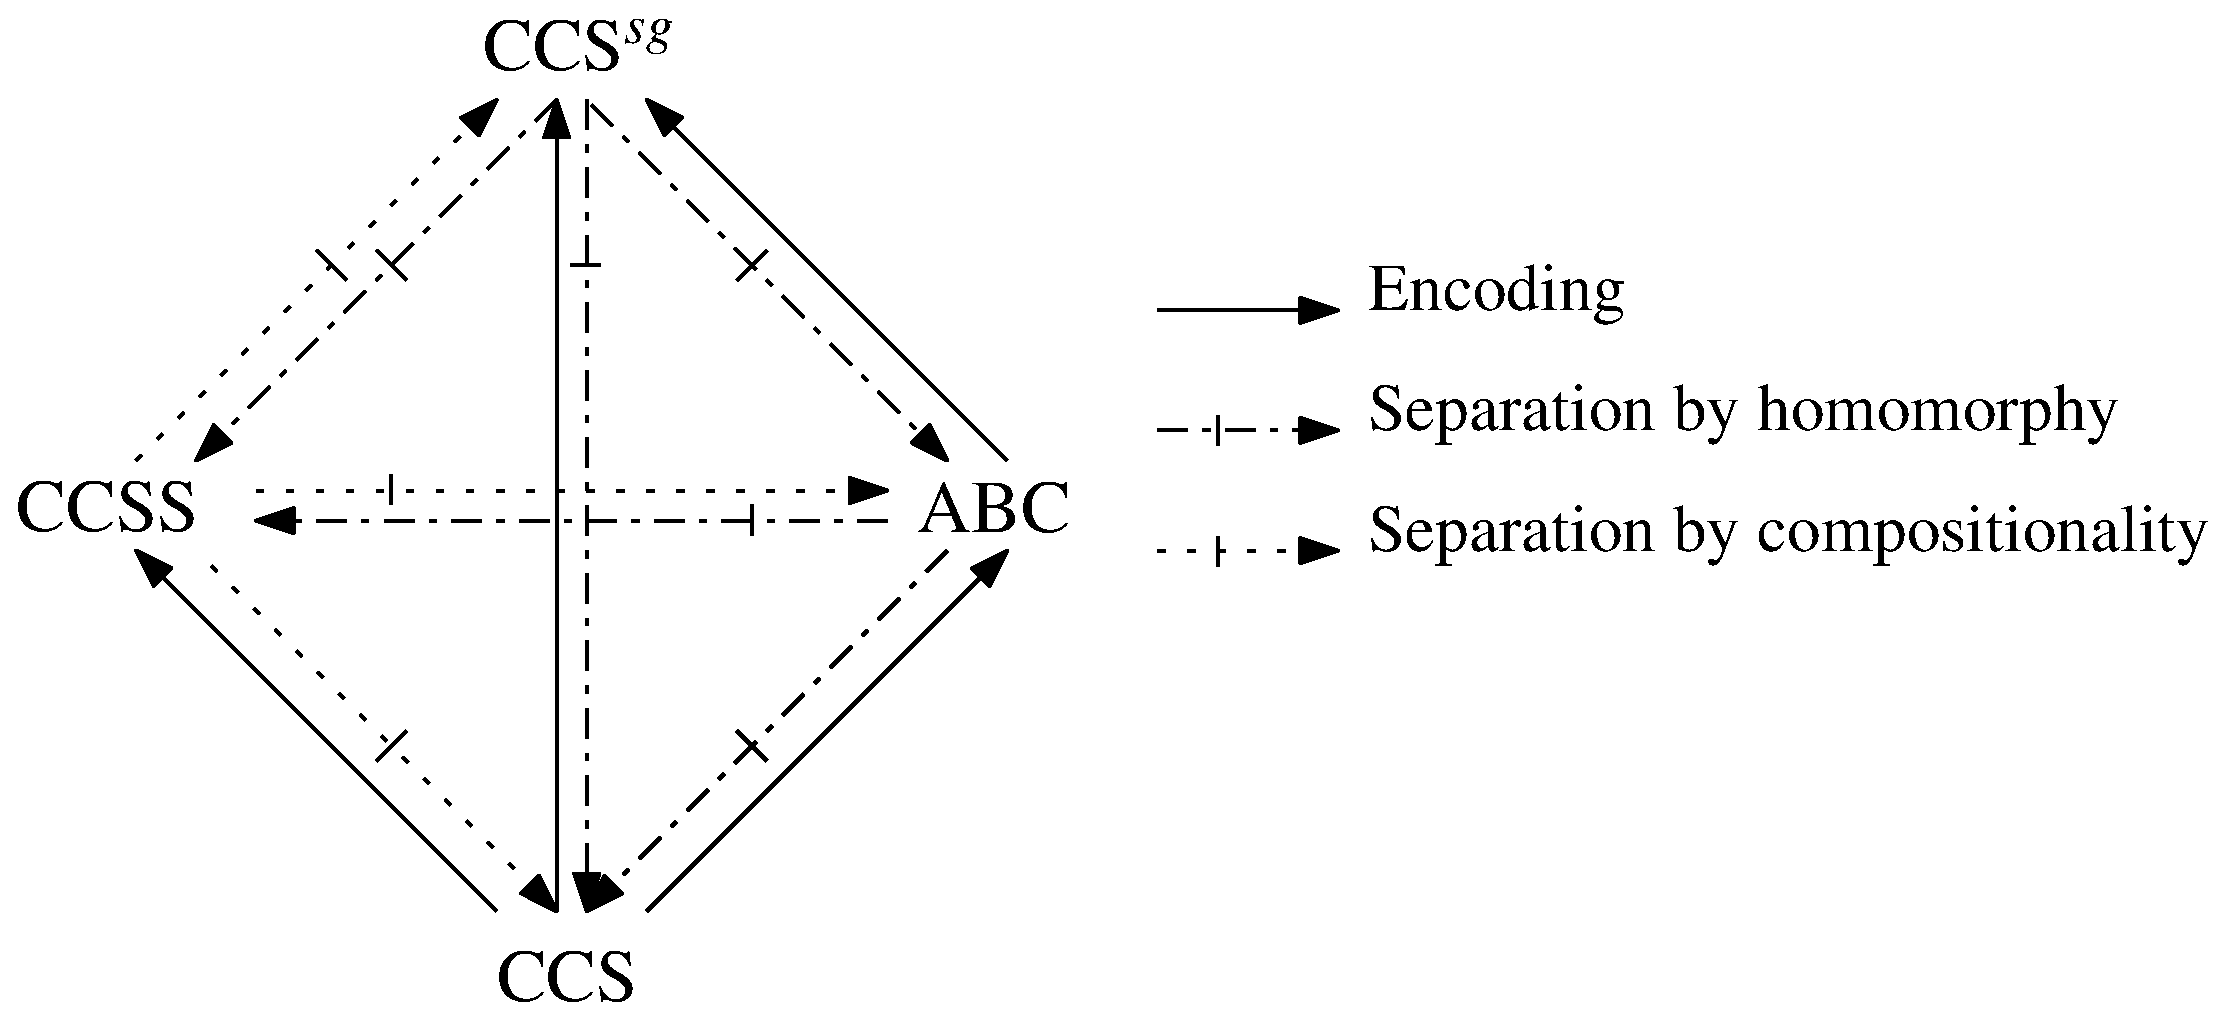
\includegraphics[width = 0.7\textwidth]{images/map.eps}
  \label{fig:map}
\end{figure}

As expected, CCS can be trivially encoded into its extensions.
These encodings respect all reasonable criteria.
The encoding from the extensions of CCS to CCS is, however, non-trivial.
The existence of a non-compositional encoding, which is supported by the fact that CCS can model $\kappa$-bounded process graphs \cite{RvG95}, is not satisfactory, as compositionality is usually required in expressiveness results, if not its stronger version homomorphy.

However, CCSS is separated from CCS if we require compositionality.
In a compositional setting, a choice operator in CCSS must be encoded into a choice operator in CCS.
As a result, we cannot encode a process in CCSS where a choice operator binds a process that does signalling into a CCS process.
The emission of a signal does not change the state of the process, hence no choice is actually made.
This mechanism of the signalling operator cannot be mimicked by CCS, neither by ABC or \CSG.

Another separation result is that ABC cannot be homomorphically encoded into CCS or CCSS.
In ABC, once a broadcast communication of a certain channel is initiated, all parallel components listening to the same channel are forced to synchronise.
The broadcast communication is summarised as one action, no matter how many parallel components participated.
In CCS and CCSS, the parallel composition is monotonic \cite{PP16}.
While homomorphically encoding a broadcast communication, we inevitably end up with a process that does more barb than intended.
The broadcast mechanism and the requirement for a homomorphic encoding separates ABC from CCS and CCSS.

This result, however, does not extend to \CSG.
In \CSG, due to different levels of priority assigned to a process, we can model a broadcast communication by preempting all other actions until the broadcast is finalised and all participating parallel components have transformed into their next states.
We presented one such encoding and proved its correctness up to a set of expressiveness criteria.

A homomorphic encoding of the backwards direction (\CSG to ABC) is, however, not existent.
Versari, Busi and Gorrieri separated \CSG from $\pi$-Calculus and $b\pi$-Calculus \cite{VBG09}.
The same process they examined as counterexample is used in this \this\ to separate \CSG from ABC.
In \CSG, we can model a process where it alone can only barb ``yes" and this process in parallel with itself can only barb ``no".
This behaviour is not preserved when we encode this process to ABC homomorphically.
When a parallel component in an ABC process barbs ``yes", we cannot prevent the whole process to also barb ``yes", which means that we have introduced unwanted behaviour which is not observed in the original ABC process.

This statement concerning parallel composition is also true for CCS and CCSS, and thus the separation result extends to CCS and CCSS.

In conclusion, the extensions of CCS are linked to CCS by encodability results on both directions, but the extensions can be separated from CCS when we require homomorphy or compositionality, respectively; ABC can be encoded into \CSG; CCSS is incomparable with both ABC and \CSG.

Strengthening the separation results in this \this\ is planned as future work.
Homomorphy is strong enough to separate priority, broadcast, and signal, but we would like to weaken it into compositionality and gain a stronger separation result, or if it is impossible, give compositional encodings between the aforementioned calculi.
Also, weak bisimulation and observation-respecting encodings are required in various works \cite{EM99, CTJ94, IP08, VBG09}, but they are still rather strong, and we plan to weaken it, or yield some reasoning that any weakening would break the result.

%%%%%%%%%%%%%%%%%%%%%%%%%%%%%%%%%%%%%%%%%%%%%%%%%%%%%%%%%%%%%%%%%%%%%%%%%%%%%%%%%%%%%%%%%%%%%%%%%%%%%%%%

\bibliographystyle{eptcsini}
\bibliography{references}

\end{document}
